\documentclass[supercite]{Experimental_Report}

\title{%
  \texorpdfstring{%
    基于大语言模型的命名实体识别方法：GPT-NER\\
    \textit{GPT-NER: Named Entity Recognition via Large Language Models}%
  }{基于大语言模型的命名实体识别方法：GPT-NER}%
}
\school{计算机科学与技术学院}
\author{瞿明睿}
\classnum{计科7班}
\stunum{U202215561}
\instructor{姚德中}

\usepackage{zhnumber}
\usepackage{tikz}
\usetikzlibrary{mindmap,trees}
\usepackage{algorithm, multirow}
\usepackage{algpseudocode}
\usepackage{amsmath}
\usepackage{amsthm}
\usepackage{framed}
\usepackage{mathtools}
\usepackage{subcaption}
\usepackage{amsmath, amssymb, amsfonts}
\usepackage{tabu}
\usepackage{xltxtra}
\usepackage{bm}
\usepackage{longtable}
\usepackage{tikz}
\usepackage{pdfpages}
\usepackage{tikzscale}
\usepackage{pgfplots}
\usepackage{graphicx}
\usepackage{xcolor}
\usepackage{booktabs}
\usepackage{makecell}

\pgfplotsset{compat=1.16}

\newcommand{\cfig}[3]{
  \begin{figure}[htb]
    \centering
    \includegraphics[width=#2\textwidth]{images/#1.tikz}
    \caption{#3}
    \label{fig:#1}
  \end{figure}
}

\newcommand{\sfig}[3]{
  \begin{subfigure}[b]{#2\textwidth}
    \includegraphics[width=\textwidth]{images/#1.tikz}
    \caption{#3}
    \label{fig:#1}
  \end{subfigure}
}

\newcommand{\xfig}[3]{
  \begin{figure}[htb]
    \centering
    #3
    \caption{#2}
    \label{fig:#1}
  \end{figure}
}

\newcommand{\rfig}[1]{\autoref{fig:#1}}
\newcommand{\ralg}[1]{\autoref{alg:#1}}
\newcommand{\rthm}[1]{\autoref{thm:#1}}
\newcommand{\rlem}[1]{\autoref{lem:#1}}
\newcommand{\reqn}[1]{\autoref{eqn:#1}}
\newcommand{\rtbl}[1]{\autoref{tbl:#1}}

\algnewcommand\Null{\textsc{null }}
\algnewcommand\algorithmicinput{\textbf{Input:}}
\algnewcommand\Input{\item[\algorithmicinput]}
\algnewcommand\algorithmicoutput{\textbf{Output:}}
\algnewcommand\Output{\item[\algorithmicoutput]}
\algnewcommand\algorithmicbreak{\textbf{break}}
\algnewcommand\Break{\algorithmicbreak}
\algnewcommand\algorithmiccontinue{\textbf{continue}}
\algnewcommand\Continue{\algorithmiccontinue}
\algnewcommand{\LeftCom}[1]{\State $\triangleright$ #1}

\newtheorem{thm}{定理}[section]
\newtheorem{lem}{引理}[section]
\renewcommand {\thefigure} {\arabic{figure}}
\colorlet{shadecolor}{black!15}

\theoremstyle{definition}
\newtheorem{alg}{算法}[section]
\def\thmautorefname~#1\null{定理~#1~\null}
\def\lemautorefname~#1\null{引理~#1~\null}
\def\algautorefname~#1\null{算法~#1~\null}

\newcommand{\tabincell}[2]{\begin{tabular}{@{}#1@{}}#2\end{tabular}}

\begin{document}

\maketitle
\clearpage

\pagenumbering{Roman}

\pagenumbering{arabic}

\begin{abstract}
尽管大规模语言模型（LLM）在多种自然语言处理任务上取得了最先进的性能，但其在命名实体识别（NER）任务上的表现仍显著低于监督式基线方法。这是由于NER任务与LLM之间的本质差异：前者本质上是序列标注任务，而后者是文本生成模型。

本文提出GPT-NER方法来解决这一问题。GPT-NER通过将序列标注任务转换为生成任务来弥合这一差距，使LLM能够轻松适配。例如，在输入文本"Columbus is a city"中查找地点实体的任务被转换为生成文本序列"@@Columbus\#\# is a city"，其中特殊标记@@\#\#用于标记待提取的实体。为了有效解决LLM的"幻觉"问题——即LLM倾向于过度自信地将空输入标记为实体——我们提出了自验证策略，通过提示LLM自问提取的实体是否属于标记的实体类型。

我们在五个广泛采用的NER数据集上进行了实验，GPT-NER达到了与完全监督基线相当的性能，据我们所知这是首次实现。更重要的是，我们发现GPT-NER在低资源和少样本设置下表现出更强的能力：当训练数据极其稀缺时，GPT-NER的性能显著优于监督模型。这证明了GPT-NER在标记样本有限的实际NER应用中的能力。
\end{abstract}

\section{引言}

大规模语言模型（LLMs）\cite{brown2020language,smith2022using,du2022glam,rae2021scaling,thoppilan2022lamda,hoffmann2022training,chowdhery2022palm,touvron2023llama}在上下文学习方面展现出了令人印象深刻的能力：仅需少量任务特定的示例作为演示，LLM就能够为新的测试输入生成结果。在上下文学习框架下，LLM在多种NLP任务中取得了令人瞩目的成果，包括机器翻译（MT）\cite{vilar2022prompting,vidal2022automatic,moslem2023adaptive}、问答（QA）\cite{robinson2022leveraging,li2022self,lazaridou2022internet}和命名实体抽取（NEE）\cite{chowdhery2022palm,brown2020language}。

尽管取得了这些进展，LLM在NER任务上的性能仍远低于监督式基线方法。这是因为NER任务与LLM之间存在本质差异：NER本质上是序列标注任务，模型需要为句子中的每个词分配实体类型标签，而LLM则是基于文本生成任务形式化的。语义标注任务与文本生成模型之间的差距导致将LLM应用于NER任务时性能较差。

本文提出GPT-NER来解决这一问题。GPT-NER将NER任务转换为LLM能够轻松适配的文本生成任务。具体而言，在输入文本"Columbus is a city"中查找地点实体的任务被转换为生成文本序列"@@Columbus\#\# is a city"，其中特殊标记@@\#\#用于标记实体。我们发现，与其他形式化方法相比，所提出的策略能够显著降低生成完全编码输入序列标签信息的文本的难度，因为模型只需要标记实体的位置并复制其余所有词元。实验表明，所提出的策略显著提升了性能。

LLM用于NER的另一个重要问题是"幻觉"问题，即LLM倾向于过度自信地将空输入标记为实体。为解决这一问题，我们提出了自验证策略，该策略置于实体抽取阶段之后，提示LLM自问提取的实体是否属于标记的实体类型。自验证策略起到调节功能，抵消LLM的过度自信，我们发现该策略在解决"幻觉"问题方面非常有效，带来了显著的性能提升。

我们在五个广泛采用的NER数据集上进行了实验，包括平面NER和嵌套NER。GPT-NER达到了与完全监督基线相当的性能，据我们所知这是首次实现。此外，我们发现当达到GPT-3的token限制时，性能尚未达到平台期，这意味着当GPT-3的4096个token限制放宽时（例如使用token限制超过20K的GPT-4），仍有提升空间。特别值得注意的是，GPT-NER在低资源和少样本NER设置下表现出令人印象深刻的能力：当训练数据极其稀缺时，GPT-NER的性能显著优于监督模型。这说明了GPT-NER在标记样本数量有限的实际NER应用中的潜力。

\section{相关工作}

\subsection{命名实体识别}

命名实体识别（NER）是一项识别文本中关键信息并将其分类为一组预定义类别的任务。解决NER的常见方法是将其形式化为序列标注任务。\cite{hammerton2003named}使用单向LSTM获取词级表示并将其输入softmax分类器获得结果。\cite{collobert2011natural}使用CNN嵌入每个输入词并利用CRF将每个嵌入解码为特定实体。\cite{chiu2016named}使用字符CNN，而\cite{devlin2018bert}使用BERT获取用于分类的词级表示。\cite{lample2016neural}将双向LSTM与CRF结合以增强预测。\cite{sarzynska2021detecting}通过大规模预训练模型提高了每个词的质量。\cite{li2019unified, li2019dice}将NER任务形式化为MRC任务，并进一步利用dice损失来提高MRC模型的性能，\cite{wang2022gnn}提出了GNN-SL模型，使通用NER模型能够在测试时参考训练示例。

\subsection{大规模语言模型与上下文学习}

大规模语言模型（LLMs）\cite{brown2020language,rae2021scaling,smith2022using,hoffmann2022training,chowdhery2022palm}在各种自然语言处理任务上获得了显著的性能提升\cite{hegselmann2022tabllm,vilar2022prompting,perez2021true,pietrzak2021story,wei2021finetuned}。使用LLM进行下游任务的策略可分为两类：微调和上下文学习。微调策略以预训练模型作为初始化，并在下游监督数据上运行额外的轮次\cite{raffel2020exploring,gururangan2018annotation,roberts2020much,guu2020retrieval}。

与微调策略不同，上下文学习（ICL）通过少样本演示提示LLM生成文本。\cite{radford2019language}首次使用包含演示的提示重新构建下游任务。\cite{brown2020language}对上下文学习进行了系统分析，并使用其GPT-3模型对各种任务进行了多项实验。\cite{chowdhery2022palm}在PaLM上对NMT任务进行了分析。\cite{perez2021true,lu2021fantastically,rubin2021learning}表明，更好的提示和演示能够带来上下文学习的性能提升。

\section{背景}
\label{background_ner}

命名实体识别（NER）是一项典型的序列标注任务，它给定句子$X=\{x_{1},...,x_{n}\}$，为每个词$x$分配一个实体类型$y\in Y$，其中$Y$表示实体标签集合，$n$表示给定句子的长度。

\subsection{NER作为序列标注任务}

解决NER的常见方法是将其形式化为序列标注任务，这可以分解为以下两个步骤：(1) 表示抽取；(2) 分类。

\paragraph{表示抽取}旨在获取输入序列中每个词元的高维表示。为了嵌入每个输入词$x$，首先将输入句子$X$送入编码器模型，例如BERT\cite{devlin2018bert}。然后使用词嵌入模型最后一层的输出作为高维表示$h_{i}\in \mathbb{R}^{m \times 1}$，其中$n$表示输入句子的长度，$m$表示向量维度变量参数。

\paragraph{分类。}对于分类，每个嵌入的高维向量$h$被送入多层感知机，然后使用softmax函数生成命名实体词汇表上的分布：
\begin{equation}
p_{\text{NER}} = \text{softmax}{\ \text{MLP}(h\in \mathbb{R}^{m \times 1})}
\end{equation}

\section{GPT-NER方法}

在本工作中，我们提出了GPT-NER，它使用大规模语言模型来解决NER任务。GPT-NER遵循上下文学习的一般范式，可以分解为三个步骤：(1) \textbf{提示构建}：对于给定的输入句子$X$，我们为$X$构建一个提示（记为$\text{Prompt}(X)$）；(2) 将构建的提示送入大语言模型（LLM）以获取生成的文本序列$W=\{w_{1},...,w_{n}\}$；(3) 将文本序列$W$转换为实体标签序列以获得最终结果。

尽管上下文学习范式简单明了，但NER任务并不直接适合它，因为它本质上是序列标注任务而非生成任务。下面我们将详细描述为适应LLM到NER任务而提出的不同策略。

\begin{figure}[htb]
    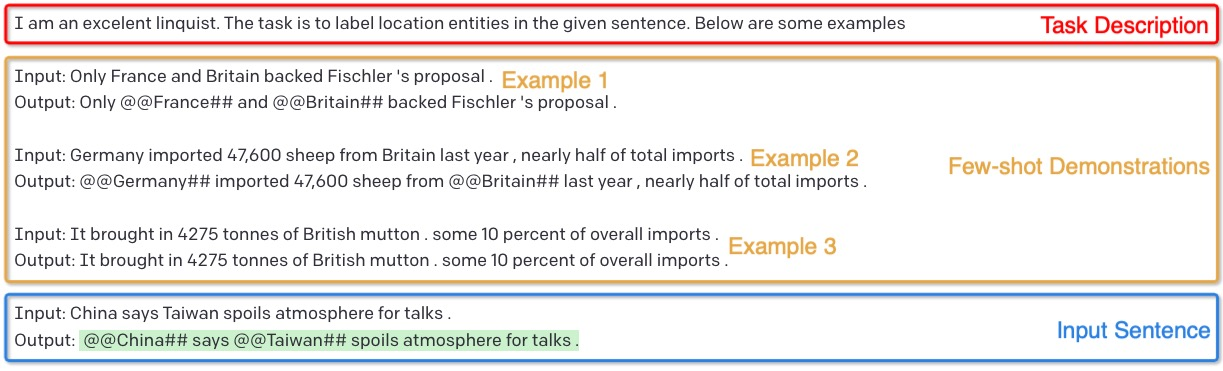
\includegraphics[scale=0.372]{images/formulation_example.jpg}
    \caption{GPT-NER提示示例。假设我们需要为给定句子"China says Taiwan spoils atmosphere for talks"识别地点实体。提示由三部分组成：\textbf{(1) 任务描述}（红色框）：指示GPT-3模型当前任务是使用语言学知识识别\textbf{地点}实体。\textbf{(2) 少样本演示}（黄色框）：为GPT-3模型提供少样本示例供参考。\textbf{(3) 输入句子}（蓝色框）：指示输入句子，GPT-3的输出为绿色。}
    \label{fig:formulation_example}
\end{figure}

\subsection{提示构建}
\label{prompt_construction}

图\ref{fig:formulation_example}是GPT-NER中使用的提示示例，它由三部分组成：

\subsubsection{任务描述}

任务描述给出任务的概述，可以进一步分解为三个组成部分：

(1) 任务描述的第一句话：

"\textit{I am an excellent linguist}"

\noindent 这是一个常量，告诉LLM使用语言学知识生成输出；

(2) 第二句话：

"\textit{The task is to label [Entity Type] entities in the given sentence}"

\noindent 这是一个可变句子，指示要提取的实体类别，\textit{[Entity Type]}表示要提取的实体类型，例如图\ref{fig:formulation_example}示例中的\textbf{地点}（Location）。值得注意的是，通过这种方式，对于每个输入句子，我们需要遍历所有实体标签，这相当于将N类分类任务转换为N个二分类任务。背后的原因如下：对于大多数当前的LLM（例如GPT-3），由于硬件限制，提示的长度有硬性限制（例如GPT-3为4096个token）。鉴于这一有限的token数量，不可能在单个提示中包含所有实体类型的描述和演示。因此，对于每个输入句子，我们构建$N$次提示，每次对应一个实体类型；

(3) 第三句话：

"\textit{Below are some examples}"

\noindent 标记描述的结束并指出少样本演示的位置。

\subsubsection{少样本演示}
\label{few_shot_demonstration}

少样本演示被附加到提示中。它有以下两个用途：(1) 它规范每个测试输入的LLM输出格式，因为LLM（很可能）会生成模仿演示格式的输出。这对于NER任务至关重要，因为我们需要输出格式一致，以便能够将自然语言形式的输出解析为NER结果；(2) 它为LLM提供关于任务的直接证据和参考以进行预测。

演示按顺序打包一系列示例，其中每个示例包括输入序列$X$和输出序列$W$：

\begin{equation}
\nonumber
    \begin{aligned}
      \textit{Input: }\text{[Example Sentence]}_{1} \\
      \textit{Output: }\text{[Labeled Sentence]}_{1} \\
      \cdots \\
      \textit{Input: }\text{[Example Sentence]}_{k} \\
      \textit{Output: }\text{[Labeled Sentence]}_{k}
    \end{aligned}
\end{equation}
其中$k$表示演示的数量。

\paragraph{LLM输出格式。}
\label{llm_format}
每个标记句子$W$的格式至关重要，它是一个文本序列，应满足以下条件：(1) 它需要包含每个词标签的信息，并能轻松转换为实体类型序列；(2) 它需要能够被LLM流畅且容易地生成，以提高模型的最终准确性。

为说明起见，这里我们先给出几个$W$形式的坏示例：对于给定的输入序列"{\it Columbus is a city}"，"{\it LOC O O O}"是$W$的直观格式，满足条件(1)；但对于条件(2)，要生成"{\it LOC O O O}"，LLM首先需要学习输入序列"{\it Columbus is a city}"中每个位置与$W$中每个位置之间的对齐关系：{\it Columbus}对应{\it LOC}，{\it is}对应{\it O}，{\it a}对应{\it O}，{\it city}对应{\it O}，这自然增加了生成任务的难度。然而，我们发现GPT-3很难生成与输入句子长度相同的输出，特别是当输入句子较长时。

为解决这一问题，我们提出LLM输出采用以下格式：如果输入序列不包含任何实体，$W$只需复制输入$X$；对于输入序列中的一个或多个实体，我们使用特殊标记"@@"和"\#\#"来包围它们。以下是提取地点（LOC）实体的示例：
\begin{equation}
\nonumber
    \begin{aligned}
      \textit{Input: }\textit{Columbus is a sailor}_{1} \\
      \textit{Output: }\textit{Columbus is a sailor}_{1} \\
      \textit{Input: }\textit{Columbus is a city}_{2} \\
      \textit{Output: }\textit{@@Columbus\#\# is a city}_{2}
    \end{aligned}
\end{equation}
所提出的策略显著弥合了序列标注任务格式与生成模型之间的差距：它显著降低了生成完全编码标签信息的文本的难度，因为LLM只需要标记实体的位置并复制其余所有词元。如我们将在消融研究部分\ref{analysis_output_format}中所示，所提出的策略相比其他格式产生了显著的性能提升。

\subsubsection{输入句子}

这部分将当前输入句子送入LLM，并期望LLM按照第\ref{llm_format}节中定义的格式生成输出序列，即：
\begin{equation}
\nonumber
    \begin{aligned}
      \textit{Input: }\text{[The Input Sentence]} \\
      \textit{Output: }
    \end{aligned}
\end{equation}
其中"\textit{Ouput:}"表示LLM开始生成标记序列的标志。

如图\ref{fig:formulation_example}底部所示，给定输入句子"\textit{China says Taiwan spoils atmosphere for talks}"，LLM\footnote{本示例中使用GPT-3。}以与前述演示相同的格式生成标记句子"\textit{@@China\#\# says @@Taiwan\#\# spoils atmosphere for talks}"，其中两个词"\textit{China}"和"\textit{Taiwan}"是被识别的\textbf{地点}实体。

至此，提示构建结束。

\begin{figure}[htb]
    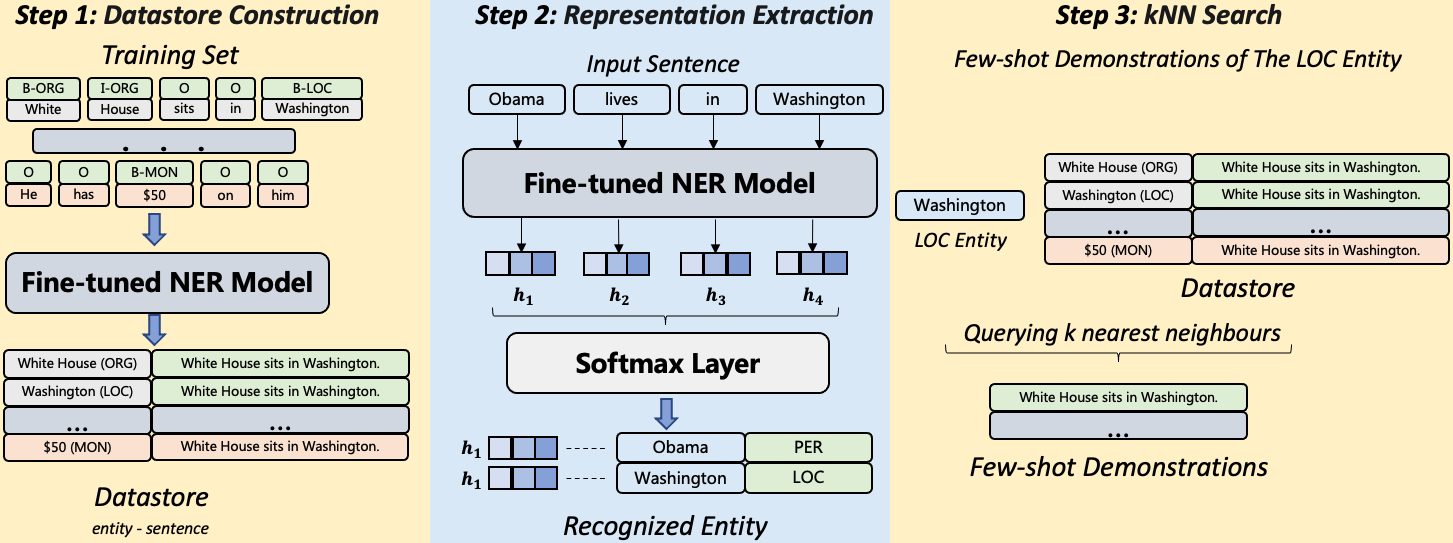
\includegraphics[scale=0.3115]{images/finetuned_method.png}
    \caption{使用实体级嵌入检索少样本演示的方法示例。假设我们需要为提示中定义了地点（LOC）实体的输入句子"Obama lives in Washington"检索少样本演示。\textbf{步骤1 数据存储构建}：我们首先使用微调的NER模型提取训练集中每个句子的实体，并将其形式化为\textit{(键, 值)}对，其中\textit{键}是提取的实体，\textit{值}是对应的句子。然后我们连接所有构建的\textit{(键, 值)}对来构建数据存储。\textbf{步骤2 表示抽取}：首先利用微调的NER模型将输入句子嵌入到高维向量序列中。然后嵌入的高维向量根据softmax层被分类为标签，其中"Obama"和"Washington"是两个被识别的实体。\textbf{步骤3 kNN搜索}：使用提取的地点实体"Washington"的嵌入作为查询，在数据存储中查找$k$个最近邻，检索到的句子被视为$k$个少样本演示。}
    \label{fig:finetuned_method}
\end{figure}

\subsection{少样本演示检索}
\label{ner_demonstration_retrieval}

这里我们描述检索演示示例的策略。

\subsubsection{随机检索}
\label{random_retrieval}

最直接的策略是从训练集中随机选择$k$个示例。缺点很明显：无法保证检索到的示例与输入语义相关。

\subsubsection{kNN检索}

为解决第\ref{random_retrieval}节中的相关性问题，我们可以从训练集中检索$k$个最近邻（$k$NN）\cite{vilar2022prompting, liu2021makes}：我们首先计算所有训练示例的表示，基于此我们获取输入测试序列的$k$个最近邻。

\paragraph{基于句子级表示的kNN。}
要在训练集中查找$k$NN示例，一种直接的方法是使用文本相似度模型如SimCSE\cite{gao2021simcse}：我们首先获取训练示例和输入序列的句子级表示，并使用余弦相似度查找$k$NN。

基于句子级表示的kNN的缺点很明显：NER是关注局部证据的词级任务，而非关注句子级语义的句子级任务。一个与输入（例如"John is a soldier"）语义相似的检索句子（例如"he is a soldier"）可能对输入中包含的NER没有帮助：在上面的例子中，检索到的句子不包含任何NER，因此没有为标记输入提供证据。

\paragraph{实体级嵌入。}
\label{entity_level_embedding}
为解决上述问题，我们需要基于词级表示而非句子级表示来检索$k$NN示例。我们首先使用微调的NER标注模型为所有训练示例的所有词元提取实体级表示作为数据存储。对于长度为$N$的给定输入序列，我们首先遍历序列中的所有词元以查找每个词元的$k$NN，获得$K\times N$个检索到的词元。接下来，我们从$K\times N$个检索到的词元中选择前$k$个词元，并使用它们关联的句子作为演示。我们在附录\ref{demonstrations_examples}中选择了几个示例来更好地说明三种检索策略的演示。

\subsection{自验证}

LLM严重受到"幻觉"或过度预测问题的影响\cite{braverman2020calibration,jiang2021can,zhao2021calibrate}。特别是在NER中，LLM倾向于过度自信地将空输入标记为实体，即使有演示。为解决这一问题，我们提出了自验证策略。给定LLM提取的实体，我们要求LLM进一步验证提取的实体是否正确，用\textit{是}或\textit{否}回答。

\begin{figure}[htb]
    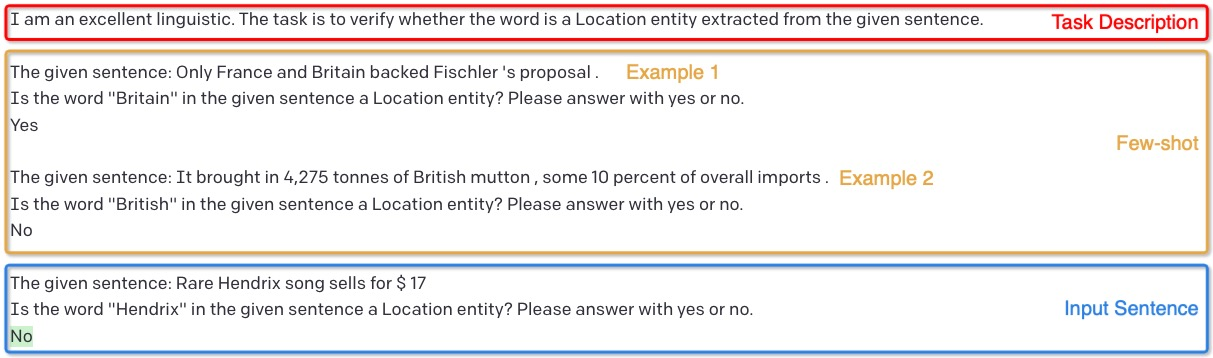
\includegraphics[scale=0.3755]{images/verify_example.jpg}
    \caption{使用GPT-3进行验证的提示示例。假设我们需要验证给定句子"Rare Hendrix song sells for \$ 17"中的词"Hendrix"是否为\textbf{地点}实体。提示由三部分组成：\textbf{(1) 任务描述}（红色框）：给出当前任务的定义——判断给定句子中指定词是否属于\textbf{地点}实体。\textbf{(2) 少样本}（黄色框）：为GPT-3提供几个示例供参考。\textbf{(3) 输入句子}（蓝色框）：指示当前需要验证的词及其所属句子，GPT-3的输出为绿色。}
    \label{fig:verification_example}
\end{figure}

我们构建了如图\ref{fig:verification_example}所示的自验证提示。以提取地点实体为例。提示以任务描述开始：

"\textit{The task is to verify whether the word is a location entity extracted from the given sentence}"。

同样，我们需要少样本演示来提高自验证器的准确性。如图\ref{fig:verification_example}中黄色框所示，每个演示由三行组成：

\noindent (1) "\textit{The input sentence: Only France and Britain backed Fischler's proposal}"，
\noindent (2) "\textit{Is the word "France" in the input sentence a location entity? Please answer with yes or no}"。
\noindent (3) \textit{Yes}。

我们在少样本设置中在提示中打包多个演示。演示后面跟着测试示例，并送入LLM以获得输出。

\paragraph{演示选择。}
我们需要为少样本自验证选择演示。由于自验证任务的核心是询问提取的实体是否为特定实体类型，我们需要选择与提取实体语义相关的训练示例，而非整体句子级语义。

因此，我们使用第\ref{entity_level_embedding}节中描述的实体级嵌入进行$k$NN演示搜索，而非句子级表示：(1) 首先，我们使用微调的NER模型为所有训练示例提取实体级表示来构建数据存储；(2) 然后，我们使用相同的微调的NER模型为查询词提取表示；(3) 最后，我们使用查询词的表示从数据存储中选择$k$个示例作为少样本演示，如果检索到的实体属于查询的实体类型，则答案为"\textit{Yes}"，否则为"\textit{no}"。

\section{实验}
\label{experiments}

我们在所有实验中使用GPT-3\cite{brown2020language}（davinci-003）作为LLM骨干。对于davinci-003参数，我们将最大输出长度设置为512个token。温度设置为0，top\_p为1，frequency\_penalty为0，presence\_penalty为0，best\_of为1。

\subsection{平面NER结果}

对于平面NER，实体不能相互重叠。我们在两个广泛使用的平面NER数据集English CoNLL2003和OntoNotes5.0上进行实验，使用span级别的精确率、召回率和F1分数作为评估指标。

\paragraph{CoNLL2003。}CoNLL2003\cite{sang2003introduction}是一个英语NER数据集，包含四种类型的命名实体：地点、组织、人物和其他，我们遵循\cite{li2019unified,ma2016end}中的协议处理数据。

\paragraph{OntoNotes5.0。}OntoNotes5.0\cite{pradhan2013towards}是一个英语NER数据集，包含18种类型的命名实体：11种类型（如人物、组织）和7种值（如日期、百分比）。两个平面NER数据集的更多详细信息（包括实体类型、句子数量和示例）见附录\ref{flat_ner_datasets_details}。

由于访问davinci-003可能很昂贵，除了完整测试集外，我们还随机选择了100个测试实例，以便社区更容易复现我们的结果。我们报告在完整测试集和部分测试集上的性能。

\begin{table}[th!]
    \centering
    \resizebox{.5\textwidth}{!}{
    \begin{tabular}{llll}\toprule
        \multicolumn{4}{c}{{\bf English CoNLL2003（采样100条）}} \\ \midrule
        \textbf{模型} & \textbf{精确率} & \textbf{召回率} & \textbf{F1} \\ \midrule
        \multicolumn{4}{c}{{\it 基线（监督模型）}} \\ \midrule
        ACE+document-context \cite{wang2020automated} & 97.8 & 98.28 & \textbf{98.04（SOTA）} \\ \midrule
        \multicolumn{4}{c}{{\it GPT-NER}} \\ \midrule
        GPT-3 + \textit{随机检索} & 88.18 & 78.54 & 83.08 \\
        GPT-3 + \textit{句子级嵌入} & 90.47 & 95 & 92.68 \\
        GPT-3 + \textit{实体级嵌入} & 94.06 & 96.54 & 95.3 \\ \midrule
        \multicolumn{4}{c}{{\it 自验证（零样本）}} \\ \midrule
        + GPT-3 + \textit{随机检索} & 88.95 & 79.73 & 84.34 \\
        + GPT-3 + \textit{句子级嵌入} & 91.77 & 96.36 & 94.01 \\
        + GPT-3 + \textit{实体级嵌入} & 94.15 & 96.77 & 95.46 \\ \midrule
        \multicolumn{4}{c}{{\it 自验证（少样本）}} \\ \midrule
        + GPT-3 + \textit{随机检索} & 90.04 & 80.14 & 85.09 \\
        + GPT-3 + \textit{句子级嵌入} & 92.92 & 95.45 & 94.17 \\
        + GPT-3 + \textit{实体级嵌入} & 94.73 & 96.97 & 95.85 \\ \bottomrule
        \multicolumn{4}{c}{{\bf English OntoNotes5.0（采样100条）}} \\ \midrule
        \textbf{模型} & \textbf{精确率} & \textbf{召回率} & \textbf{F1} \\ \midrule
        \multicolumn{4}{c}{{\it 基线（监督模型）}} \\ \midrule
        BERT-MRC+DSC \cite{li2019dice} & 93.81 & 93.95 & \textbf{93.88（SOTA）} \\ \midrule
        \multicolumn{4}{c}{{\it GPT-NER}} \\ \midrule
        GPT-3 + \textit{随机检索} & 64.21 & 65.51 & 64.86 \\
        GPT-3 + \textit{句子级嵌入} & 76.08 & 83.06 & 79.57 \\
        GPT-3 + \textit{实体级嵌入} & 78.38 & 83.9 & 81.14 \\ \midrule
        \multicolumn{4}{c}{{\it 自验证（零样本）}} \\ \midrule
        + GPT-3 + \textit{随机检索} & 64.94 & 65.90 & 65.42 \\
        + GPT-3 + \textit{句子级嵌入} & 77.33 & 83.29 & 80.31 \\
        + GPT-3 + \textit{实体级嵌入} & 79.05 & 83.71 & 81.38 \\ \midrule
        \multicolumn{4}{c}{{\it 自验证（少样本）}} \\ \midrule
        + GPT-3 + \textit{随机检索} & 65.21 & 66.25 & 65.73 \\
        + GPT-3 + \textit{句子级嵌入} & 77.64 & 83.22 & 80.43 \\
        + GPT-3 + \textit{实体级嵌入} & 79.25 & 83.73 & 81.49 \\ \bottomrule
    \end{tabular}
    }
     \caption{两个\textbf{平面}NER数据集CoNLL2003和OntoNotes5.0的采样100条数据结果。}
    \label{tab:sample_ner_result}
\end{table}

\begin{table}[th!]
    \centering
    \resizebox{.5\textwidth}{!}{
    \begin{tabular}{llll}\toprule
        \multicolumn{4}{c}{{\bf English CoNLL2003（完整数据集）}} \\ \midrule
        \textbf{模型} & \textbf{精确率} & \textbf{召回率} & \textbf{F1} \\ \midrule
        \multicolumn{4}{c}{{\it 基线（监督模型）}} \\ \midrule
        BERT-Tagger \cite{devlin2018bert} & - & - & 92.8 \\
        BERT-MRC \cite{li2019unified} & 92.33 & 94.61 & 93.04 \\
        GNN-SL \cite{wang2022gnn} & 93.02 & 93.40  & 93.2 \\
        ACE+document-context \cite{wang2020automated} & - & - & \textbf{94.6（SOTA）} \\ \midrule
        \multicolumn{4}{c}{{\it GPT-NER}} \\ \midrule
        GPT-3 + \textit{随机检索} & 77.04 & 68.69 & 72.62 \\
        GPT-3 + \textit{句子级嵌入} & 81.04 & 88.00 & 84.36 \\
        GPT-3 + \textit{实体级嵌入} & 88.54 & 91.4 & 89.97 \\ \midrule
        \multicolumn{4}{c}{{\it 自验证（零样本）}} \\ \midrule
        + GPT-3 + \textit{随机检索} & 77.13 & 69.23 & 73.18 \\
        + GPT-3 + \textit{句子级嵌入} & 83.31 & 88.11 & 85.71 \\
        + GPT-3 + \textit{实体级嵌入} & 89.47 & 91.77 & 90.62 \\ \midrule
        \multicolumn{4}{c}{{\it 自验证（少样本）}} \\ \midrule
        + GPT-3 + \textit{随机检索} & 77.50 & 69.38 & 73.44 \\
        + GPT-3 + \textit{句子级嵌入} & 83.73 & 88.07 & 85.9 \\
        + GPT-3 + \textit{实体级嵌入} & 89.76 & 92.06 & 90.91 \\ \bottomrule
        \multicolumn{4}{c}{{\bf English OntoNotes5.0（完整数据集）}} \\ \midrule
        \textbf{模型} & \textbf{精确率} & \textbf{召回率} & \textbf{F1} \\ \midrule
        \multicolumn{4}{c}{{\it 基线（监督模型）}} \\ \midrule
        BERT-Tagger \cite{devlin2018bert} & 90.01 & 88.35 & 89.16 \\
        BERT-MRC \cite{li2019unified} & 92.98 & 89.95 & 91.11 \\
        GNN-SL \cite{wang2022gnn} & 91.48 & 91.29  & 91.39 \\
        BERT-MRC+DSC \cite{li2019dice} & 91.59 & 92.56 & \textbf{92.07（SOTA）} \\ \midrule
        \multicolumn{4}{c}{{\it GPT-NER}} \\ \midrule
        GPT-3 + \textit{随机检索} & 58.8 & 64.36 & 61.58 \\
        GPT-3 + \textit{句子级嵌入} & 71.87 & 78.77 & 75.32 \\
        GPT-3 + \textit{实体级嵌入} & 79.17 & 84.29 & 81.73 \\ \midrule
        \multicolumn{4}{c}{{\it 自验证（零样本）}} \\ \midrule
        + GPT-3 + \textit{随机检索} & 59.14 & 64.44 & 61.79 \\
        + GPT-3 + \textit{句子级嵌入} & 72.29 & 78.81 & 75.55 \\
        + GPT-3 + \textit{实体级嵌入} & 79.64 & 84.52 & 82.08 \\ \midrule
        \multicolumn{4}{c}{{\it 自验证（少样本）}} \\ \midrule
        + GPT-3 + \textit{随机检索} & 59.23 & 64.65 & 61.94 \\
        + GPT-3 + \textit{句子级嵌入} & 72.35 & 78.79 & 75.57 \\
        + GPT-3 + \textit{实体级嵌入} & 79.89 & 84.51 & 82.20 \\ \bottomrule
    \end{tabular}
    }
     \caption{两个\textbf{平面}NER数据集CoNLL2003和OntoNotes5.0的完整数据集结果。}
    \label{tab:ner_result}
\end{table}

\paragraph{基线方法。}我们采用当前广泛使用的NER系统作为基线，包括：
\begin{itemize}
  \item \textbf{BERT-Tagger}\cite{devlin2018bert}：在完整训练数据集上微调BERT。
  \item \textbf{MRC-NER}\cite{li2019unified}：将NER任务形式化为机器阅读理解（MRC）任务，并在完整训练数据集上训练MRC-NER模型。
  \item \textbf{MRC-NER+DSC}\cite{li2019dice}：OntoNotes5.0数据集上的当前SOTA模型，在训练期间使用dice损失替代标准交叉熵损失。
  \item \textbf{GNN-SL}\cite{wang2022gnn}：在完整训练数据集上微调RoBERTa\cite{liu2019roberta}，并使用GNN在测试时参考整个训练示例。
  \item \textbf{ACE+document-context}\cite{wang2020automated}：CoNLL2003数据集上的当前SOTA模型，在完整训练数据集上优化控制器以找到更好的嵌入连接。
\end{itemize}

\paragraph{主要结果。}
\label{flat_ner_results}
表\ref{tab:sample_ner_result}和表\ref{tab:ner_result}分别显示了平面NER在部分测试集和完整测试集上的结果。观察结果如下：

(1) $k$NN检索对NER任务至关重要。对于随机检索策略（演示是随机选择而非通过$k$NN搜索），在完整CoNLL2003和OntoNotes5.0集上的性能仅为72.62和61.58。当使用句子级嵌入进行$k$NN演示检索时，完整CoNLL2003和OntoNotes5.0上的结果飙升至84.36和75.32。

(2) 我们观察到，通过将句子级嵌入更改为用于$k$NN演示搜索的词级嵌入，获得了显著改进：CoNLL2003数据集上84.36对89.97，OntoNotes5.0上75.32对81.73。这一现象的原因是NER是关注局部证据的词级任务，而非关注句子级语义的句子级任务：两个句子"he is a soldier"和"John is a soldier"语义相似但不共享任何相同实体。使用词级表示进行$k$NN搜索有助于检索与特定实体类型更相关的演示，从而获得更好的性能。

(3) 我们通过添加自验证观察到进一步的改进：在完整CoNLL2003数据集上使用实体级嵌入，不使用自验证和使用自验证的性能分别为89.97对90.62（零样本学习）和84.97对85.91（少样本学习）。结果证明了自验证在缓解GPT-3过度预测方面的有效性。

(4) 基于LLM的系统获得了与使用BERT的监督基线相当的结果，即完整CoNLL2003数据集上90.91对92.8，完整OntoNotes5.0数据集上82.20对89.16。我们观察到与监督SOTA模型之间仍存在差距：完整CoNLL2003数据集上94.6对90.91，完整OntoNotes5.0数据集上92.07对82.20。如消融研究部分所示，我们发现当达到GPT-3的token限制时，性能尚未达到平台期。这意味着当token限制放宽时（例如使用GPT-4，其token限制超过20K），仍有提升空间。当GPT-4 API可访问时，我们将更新性能。

\subsection{嵌套NER结果}

对于嵌套NER，每个句子中的实体可能相互重叠，如下例所示：
\begin{equation}
\nonumber
    \begin{aligned}
      \textit{Sentence}\text{: The Chinese embassy in France}\\
      \textit{Geographical Political Entities}\text{: Chinese, France}\\
      \textit{Facility Entities}\text{: The Chinese embassy in France}
    \end{aligned}
\end{equation}
其中两个地理政治实体"\textit{Chinese}"和"\textit{France}"与设施实体"\textit{The Chinese embassy in France}"重叠。

我们在三个广泛使用的嵌套NER数据集上进行实验：ACE2004、ACE2005和GENIA，并使用span级别的精确率、召回率和F1分数进行评估。

\paragraph{ACE2004和ACE2005。}
ACE2004\cite{doddington2004automatic}和ACE2005\cite{christopher2006ace}包含七种实体类型（如组织实体和人物实体）。我们遵循\cite{katiyar2018nested}中普遍采用的协议处理这两个数据集，将它们按8:1:1的比例划分为训练集、开发集和测试集。

\paragraph{GENIA。}
GENIA\cite{ohta2002genia}是一个分子生物学领域的英语嵌套NER数据集，包含五种实体类型（如DNA和RNA）。三个嵌套NER数据集ACE2004、ACE2005和GENIA的更多详细信息（包括实体类型、句子数量和示例）见附录\ref{nested_ner_datasets_details}。

\paragraph{基线方法。}对于基线，我们包含四个广泛使用的监督模型：
\begin{itemize}
\item \textbf{BERT-MRC}\cite{li2019unified}：GENIA数据集上的当前SOTA模型，将NER任务形式化为机器阅读理解（MRC）任务，并在完整训练数据集上训练MRC-NER模型。
\item \textbf{Triaffine+BERT}\cite{yuan2021fusing}：在完整训练集上微调BERT\cite{devlin2018bert}，并融合异构因素进行span表示和分类。
\item \textbf{Triaffine+ALBERT}\cite{yuan2021fusing}：在完整训练集上微调ALBERT\cite{lan2019albert}，并融合异构因素进行span表示和分类。
\item \textbf{BINDER}\cite{zhang2022optimizing}：ACE2004数据集和ACE2005数据集上的当前SOTA模型，利用双编码器框架应用对比学习将候选文本span和实体类型映射到相同的向量表示空间进行表示和分类。
\end{itemize}

\begin{table}[th!]
    \centering
    \resizebox{.5\textwidth}{!}{
    \begin{tabular}{llll}\toprule
        \multicolumn{4}{c}{{\bf ACE2004（完整数据集）}} \\ \midrule
        \textbf{模型} & \textbf{精确率} & \textbf{召回率} & \textbf{F1} \\ \midrule
        \multicolumn{4}{c}{{\it 基线（监督模型）}} \\ \midrule
        BERT-MRC \cite{li2019unified} & 85.05 & 86.32 & 85.98 \\
        Triaffine+BERT \cite{yuan2021fusing} & 87.13 & 87.68 & 87.40 \\
        Triaffine+ALBERT \cite{yuan2021fusing} & 88.88 & 88.24 & 88.56 \\
        BINDER \cite{zhang2022optimizing} & 88.3 & 89.1 & \textbf{88.7（SOTA）} \\ \midrule
        \multicolumn{4}{c}{{\it GPT-NER}} \\ \midrule
        GPT-3 + \textit{随机检索} & 55.04 & 41.76 & 48.4 \\
        GPT-3 + \textit{句子级嵌入} & 65.31 & 53.67 & 60.68 \\
        GPT-3 + \textit{实体级嵌入} & 72.23 & 75.01 & 73.62 \\ \midrule
        \multicolumn{4}{c}{{\it 自验证（零样本）}} \\ \midrule
        GPT-3 + \textit{随机检索} & 55.44 & 42.22 & 48.83 \\
        GPT-3 + \textit{句子级嵌入} & 69.64 & 54.98 & 62.31 \\
        GPT-3 + \textit{实体级嵌入} & 73.58 & 74.74 & 74.16 \\ \midrule
        \multicolumn{4}{c}{{\it 自验证（少样本）}} \\ \midrule
        GPT-3 + \textit{随机检索} & 55.63 & 42.49 & 49.06 \\
        GPT-3 + \textit{句子级嵌入} & 70.17 & 54.87 & 62.52 \\
        GPT-3 + \textit{实体级嵌入} & 73.29 & 75.11 & 74.2 \\ \bottomrule
        \multicolumn{4}{c}{{\bf ACE2005（完整数据集）}} \\ \midrule
        \textbf{模型} & \textbf{精确率} & \textbf{召回率} & \textbf{F1} \\ \midrule
        \multicolumn{4}{c}{{\it 基线（监督模型）}} \\ \midrule
        Triaffine+BERT \cite{yuan2021fusing} & 86.70 & 86.94 & 86.82 \\
        BERT-MRC \cite{li2019unified} & 87.16 & 86.59 & 86.88 \\
        Triaffine+ALBERT \cite{yuan2021fusing} & 87.39 & 90.31 & 88.83 \\
        BINDER \cite{zhang2022optimizing} & 89.1 & 89.8 & \textbf{89.5（SOTA）} \\ \midrule
        \multicolumn{4}{c}{{\it GPT-NER}} \\ \midrule
        GPT-3 + \textit{随机检索} & 45.5 & 46.24 & 45.37 \\
        GPT-3 + \textit{句子级嵌入} & 58.04 & 58.97 & 58.50 \\
        GPT-3 + \textit{实体级嵌入} & 71.72 & 74.2 & 72.96 \\ \midrule
        \multicolumn{4}{c}{{\it 自验证（零样本）}} \\ \midrule
        GPT-3 + \textit{随机检索} & 45.06 & 46.62 & 45.84 \\
        GPT-3 + \textit{句子级嵌入} & 59.49 & 60.17 & 59.83 \\
        GPT-3 + \textit{实体级嵌入} & 72.63 & 75.39 & 73.46 \\ \midrule
        \multicolumn{4}{c}{{\it 自验证（少样本）}} \\ \midrule
        GPT-3 + \textit{随机检索} & 45.49 & 46.73 & 46.11 \\
        GPT-3 + \textit{句子级嵌入} & 59.69 & 60.35 & 60.02 \\
        GPT-3 + \textit{实体级嵌入} & 72.77 & 75.51 & 73.59 \\ \midrule
        \multicolumn{4}{c}{{\bf GENIA（完整数据集）}} \\ \midrule
        \textbf{模型} & \textbf{精确率} & \textbf{召回率} & \textbf{F1} \\ \midrule
        \multicolumn{4}{c}{{\it 基线（监督模型）}} \\ \midrule
        Triaffine+BERT \cite{yuan2021fusing} & 80.42 & 82.06 & 81.23 \\
        BERT-MRC \cite{li2019unified} & 85.18 & 81.12 & \textbf{83.75（SOTA）} \\ \midrule
        \multicolumn{4}{c}{{\it GPT-NER}} \\ \midrule
        GPT-3 + \textit{随机检索} & 44.1 & 38.64 & 41.37 \\
        GPT-3 + \textit{句子级嵌入} & 63.43 & 44.17 & 51.68 \\
        GPT-3 + \textit{实体级嵌入} & 61.38 & 66.74 & 64.06 \\ \midrule
        \multicolumn{4}{c}{{\it 自验证（零样本）}} \\ \midrule
        GPT-3 + \textit{随机检索} & 44.31 & 38.79 & 41.55 \\
        GPT-3 + \textit{句子级嵌入} & 59.54 & 44.26 & 51.9 \\
        GPT-3 + \textit{实体级嵌入} & 61.77 & 66.81 & 64.29 \\ \midrule
        \multicolumn{4}{c}{{\it 自验证（少样本）}} \\ \midrule
        GPT-3 + \textit{随机检索} & 44.68 & 38.98 & 41.83 \\
        GPT-3 + \textit{句子级嵌入} & 59.87 & 44.39 & 52.13 \\
        GPT-3 + \textit{实体级嵌入} & 61.89 & 66.95 & 64.42 \\ \bottomrule
    \end{tabular}
    }
     \caption{三个\textbf{嵌套}NER数据集ACE2004、ACE2005和GENIA的完整数据集结果。}
    \label{tab:nest_ner_result}
\end{table}

\paragraph{主要结果。}

结果显示在表\ref{tab:nest_ner_result}中，观察到的现象与平面NER相似：

(1) 再次，$k$NN检索至关重要：在完整ACE2004数据集上，随机检索为48.4，而使用KNN搜索的实体级嵌入检索为73.62。

(2) 对于$k$NN演示搜索，通过将句子级嵌入更改为实体级嵌入获得了显著改进：ACE2004上60.68对73.62，GENIA上56.68对69.06。

(3) 通过添加自验证获得了进一步的性能提升，即在完整ACE2004数据集上使用句子级嵌入，零样本学习为60.68对62.31，少样本学习为60.68对62.52。

我们还观察到，GPT-NER与SOTA模型之间的差距大于平面NER。这是因为：

(1) 嵌套NER数据集包含更多相似的实体类型，例如地点实体（LOC）和地理实体（GPE）。由于只允许有限数量的演示，GPT-3更难区分它们。

(2) 三个嵌套NER数据集的标注指南更复杂且不够直接。例如，句子"\textit{The bodies of six people were found in the region}"中的子串"\textit{The bodies of six people}"被标注为人物实体。对于在完整训练集上微调的监督模型来说，学习这些复杂规则更容易，而对于仅有有限数量演示的LLM模型来说则困难得多。

\begin{figure}[htb]
    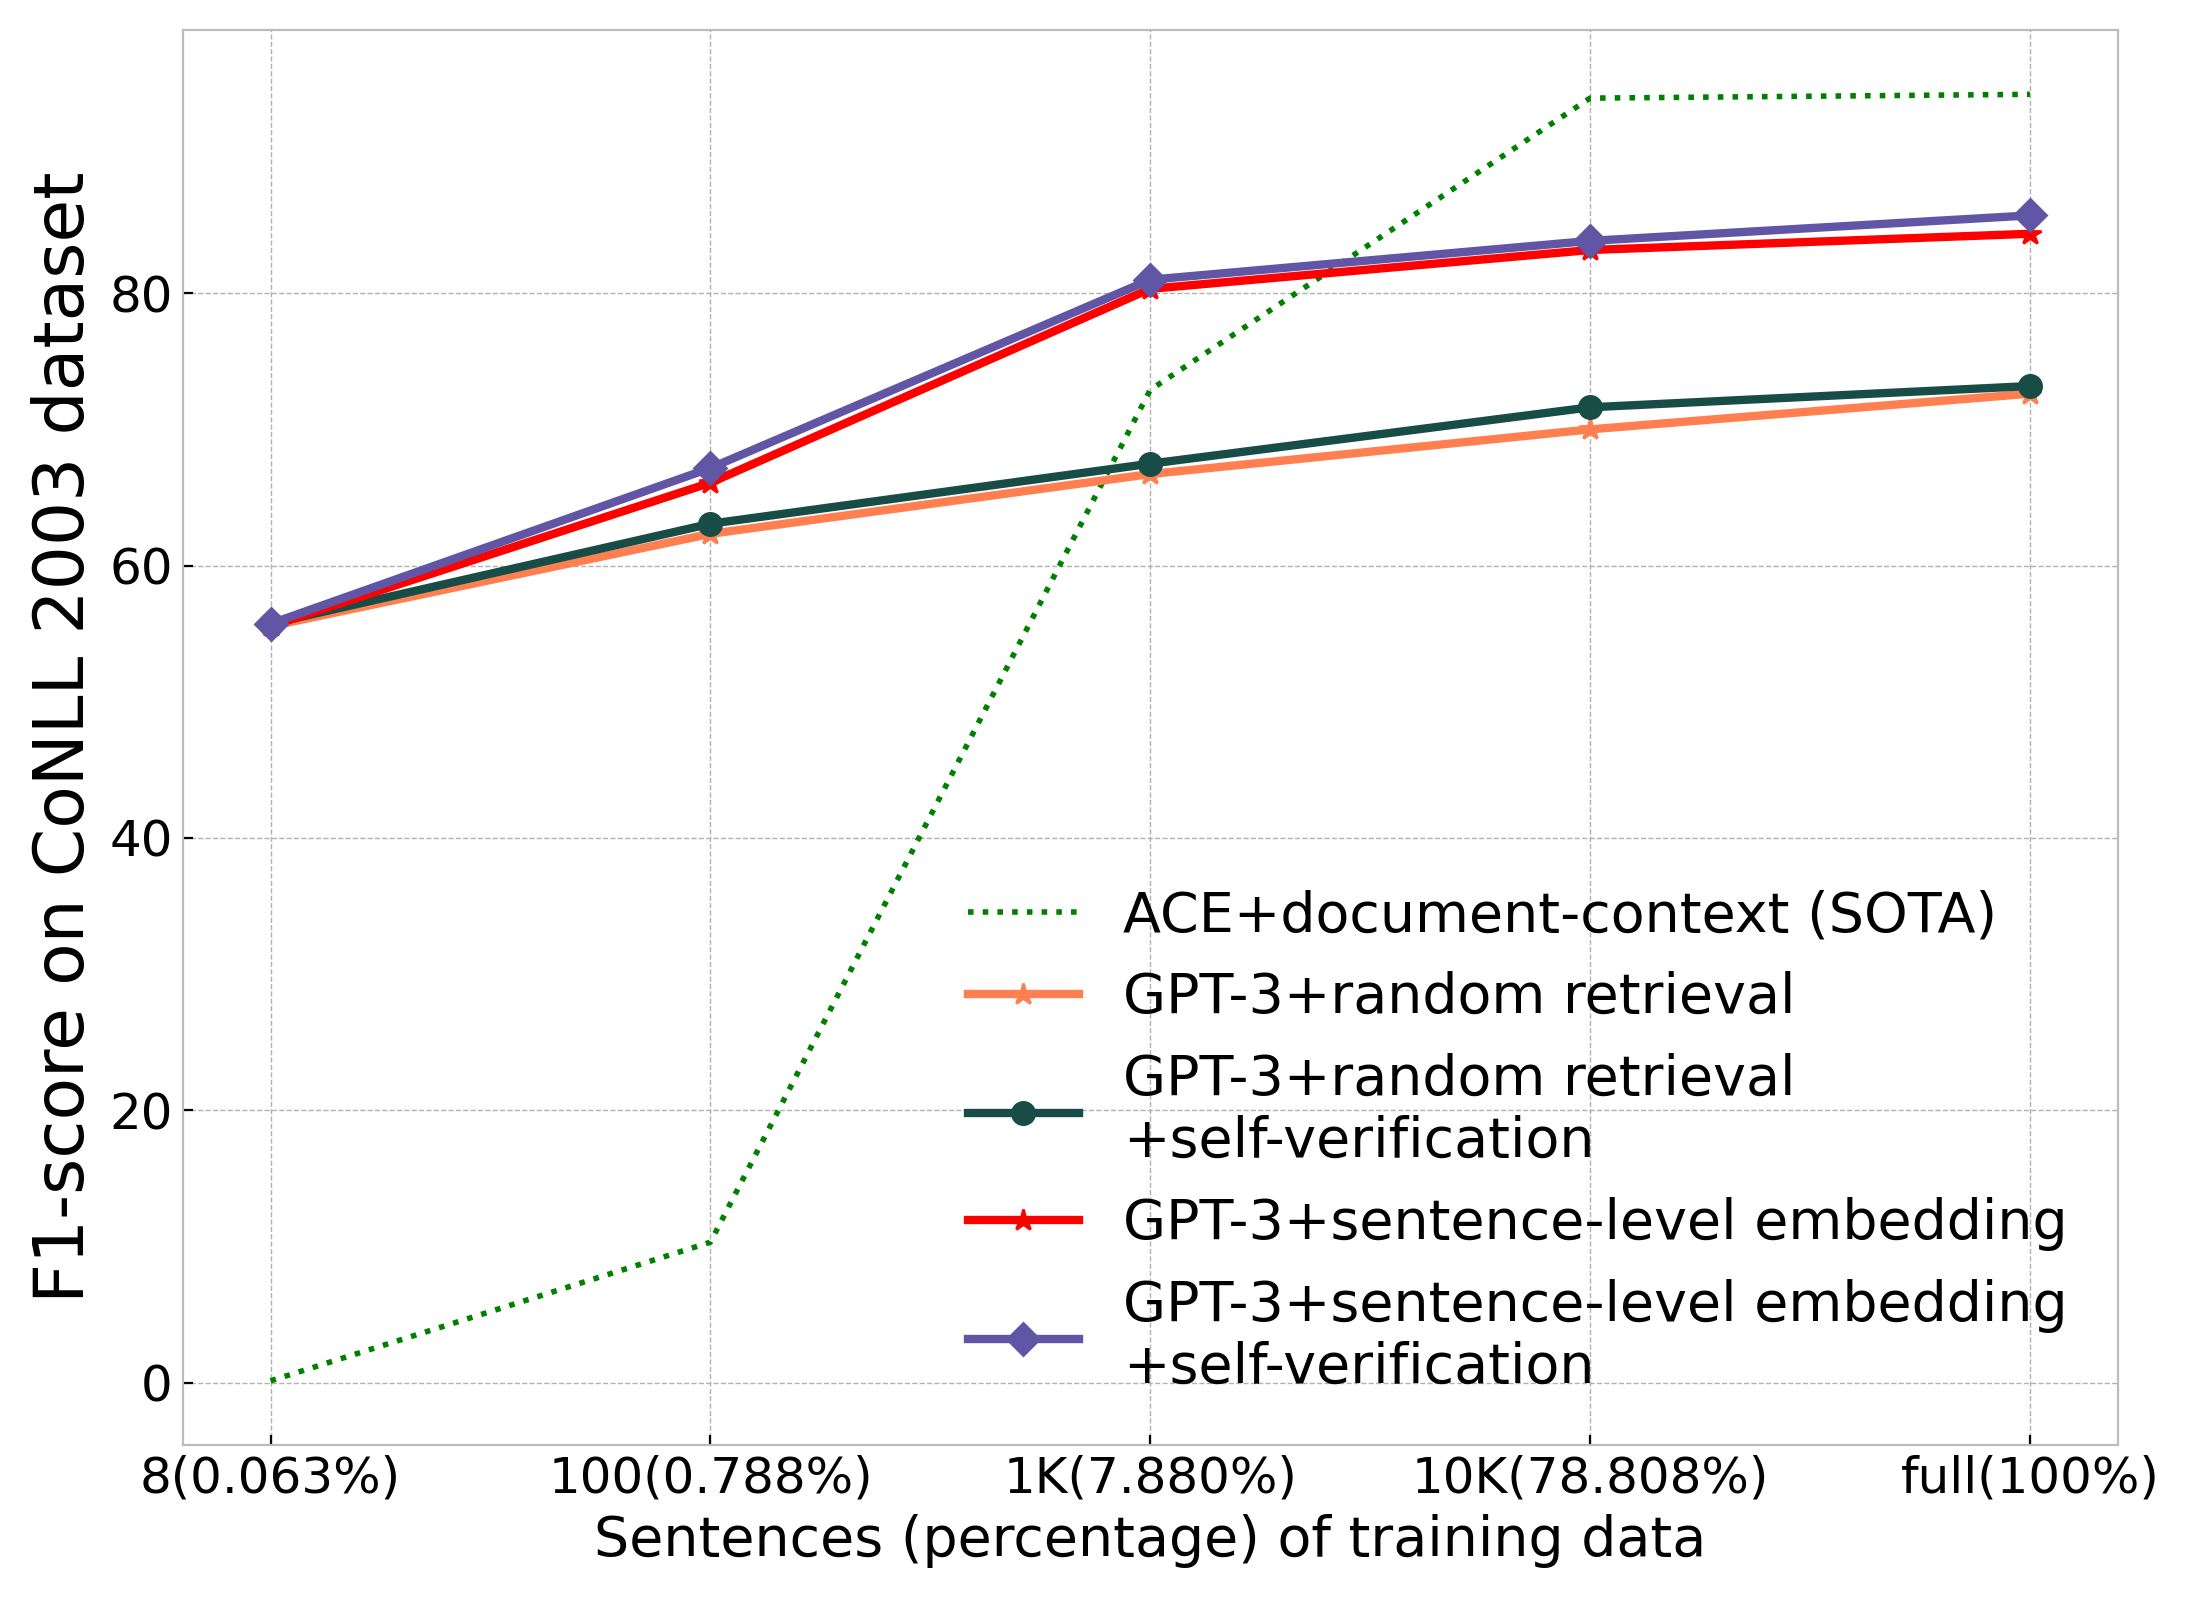
\includegraphics[scale=0.285]{images/low_resource.png}
    \caption{CoNLL2003数据集上的低资源对比。}
    \label{fig:low_resource}
\end{figure}

\subsection{低资源场景结果}

我们进行实验以估计GPT-NER在低资源设置下的性能。为了模拟低资源场景，我们随机选择完整训练数据的子集作为训练集：(a) 8个训练句子（$0.063\%$）；(b) 100个训练句子（$0.788\%$）；(c) 1K个句子（$7.880\%$）；(d) 10K个句子（$78.808\%$）。对于8个训练句子的设置，数据集被构造为确保每种实体类型包含一个正例和一个负例。评估在完整测试集上进行。

\paragraph{实验设置。}
我们使用与第\ref{experiments}节相同的GPT参数。对于基线，我们在不同的训练子集上训练ACE模型\cite{wang2020automated}（当前SOTA模型）。对于GPT-NER，我们在少样本学习阶段使用随机演示检索和基于句子级嵌入的演示检索进行演示选择。对于自验证阶段，我们只使用不需要演示的零样本学习。

\subsubsection{结果}
结果显示在图\ref{fig:low_resource}中。观察结果如下：

(1) 当训练集大小极小时（即8或100个句子），监督模型的性能远低于GPT-3。具体而言，仅用8个训练示例，GPT-NER的F1分数已经达到约60，而监督模型的性能约为0。这证明了GPT-NER在低资源设置下比监督基线具有显著更好的泛化能力。

(2) 随着训练数据的增加，KNN搜索的性能增长快于随机检索，这符合我们的预期：对于随机检索，所有演示都是随机选择的，增加训练数据规模的影响最小：从100个和1000个集合中选择K个演示的结果相似，因为它们都是随机选择的。但对于$k$NN演示搜索，增加训练数据规模意味着选择的演示更有可能与输入相关，从而获得更好的性能。

(3) 当数据量达到$10\%$时，随着训练数据规模的增加，监督模型的性能将显著提高，而GPT-3的结果将小幅增加。这一现象表明，对于上下文学习，与其专注于增加训练数据量，不如专注于提高检索演示的质量（例如从随机检索到基于$k$NN的检索）和提示结构（例如添加自验证）。

\section{消融研究}

\subsection{LLM输出格式的变化}
\label{analysis_output_format}

在第\ref{llm_format}节中，我们提出使用特殊标记"@@"和"\#\#"来规范GPT-3输出的格式，例如，"\textit{@@Columbus\#\# is a city}"表示词"\textit{Columbus}"是被识别的实体。我们将所提出的输出格式与以下两种格式进行比较：

\paragraph{BMES}直接输出输入中每个词元的开始、中间、结束和单例指示符：
\begin{equation}
\nonumber
    \begin{aligned}
      \textit{Input}\text{:White House is in Washington}\\
      \textit{Output}\text{:B-ORG E-ORG O O O}
    \end{aligned}
\end{equation}

\paragraph{Entity+Position}要求LLM输出句子中的实体及其位置：
\begin{equation}
\nonumber
    \begin{aligned}
      \textit{Input}\text{:White House is in Washington}\\
      \textit{Output}\text{:White House (0)}
    \end{aligned}
\end{equation}
其中"White House (0)"表示"\text{White House}"是一个实体，其在输入句子中的起始位置为0。

为了实现公平比较，我们对三种输出格式使用相同的设置，并在100样本CoNLL 2003数据集上进行32少样本实验。

所提出的\#\#@@策略、{\it BMES}和{\it Entity+Position}的F1分数分别为92.68、29.75和38.73，其中{\it BMES}和{\it Entity+Position}显著低于所提出的\#\#@@策略。解释如下：对于\textbf{BMES}策略，LLM需要学习每个输入词与每个\textbf{BMES}标签之间的对齐关系：\textit{White}对应\textit{B-ORG}，\textit{House}对应\textit{E-ORG}，\textit{is}对应\textit{O}，\textit{in}对应\textit{O}，\textit{Washington}对应\textit{O}。通过分析错误样本，我们发现LLM甚至很难输出与输入句子长度相同的BMES字符串，特别是当输入句子较长时，导致最终评估性能较差。

对于\textbf{Entity+Position}策略，我们发现LLM通常混淆位置索引的含义（例如，它是字符索引还是词索引），导致实体位置不正确。这个问题可以通过演示部分缓解，但考虑到GPT-3的4096个token限制仍然存在。不正确的位置索引使得将输出文本映射到序列标注评估格式变得困难，导致最终评估性能较差。

\subsection{少样本演示数量的影响}

我们进行实验以估计演示数量的影响。实验在100样本CoNLL 2003数据集上进行。结果显示在图\ref{fig:k_shot_demonstrations}中。我们可以观察到，随着$k$的增加，所有三种基于LLM的结果都持续上升。当我们接近4096个token的演示限制时，结果仍未达到平台期。这意味着如果允许更多演示，性能仍会上升。

观察到一个有趣的现象，当演示数量较少时，即$k=2,4$，基于$k$NN的策略表现不如随机检索策略。解释如下：基于$k$NN的检索倾向于选择与输入句子非常相似的演示。因此，如果输入句子不包含任何实体，检索到的演示也很可能不包含实体。在这种情况下，演示不包含我们希望强制执行的输出格式信息，导致LLM输出任意格式。

\begin{figure}[htb]
    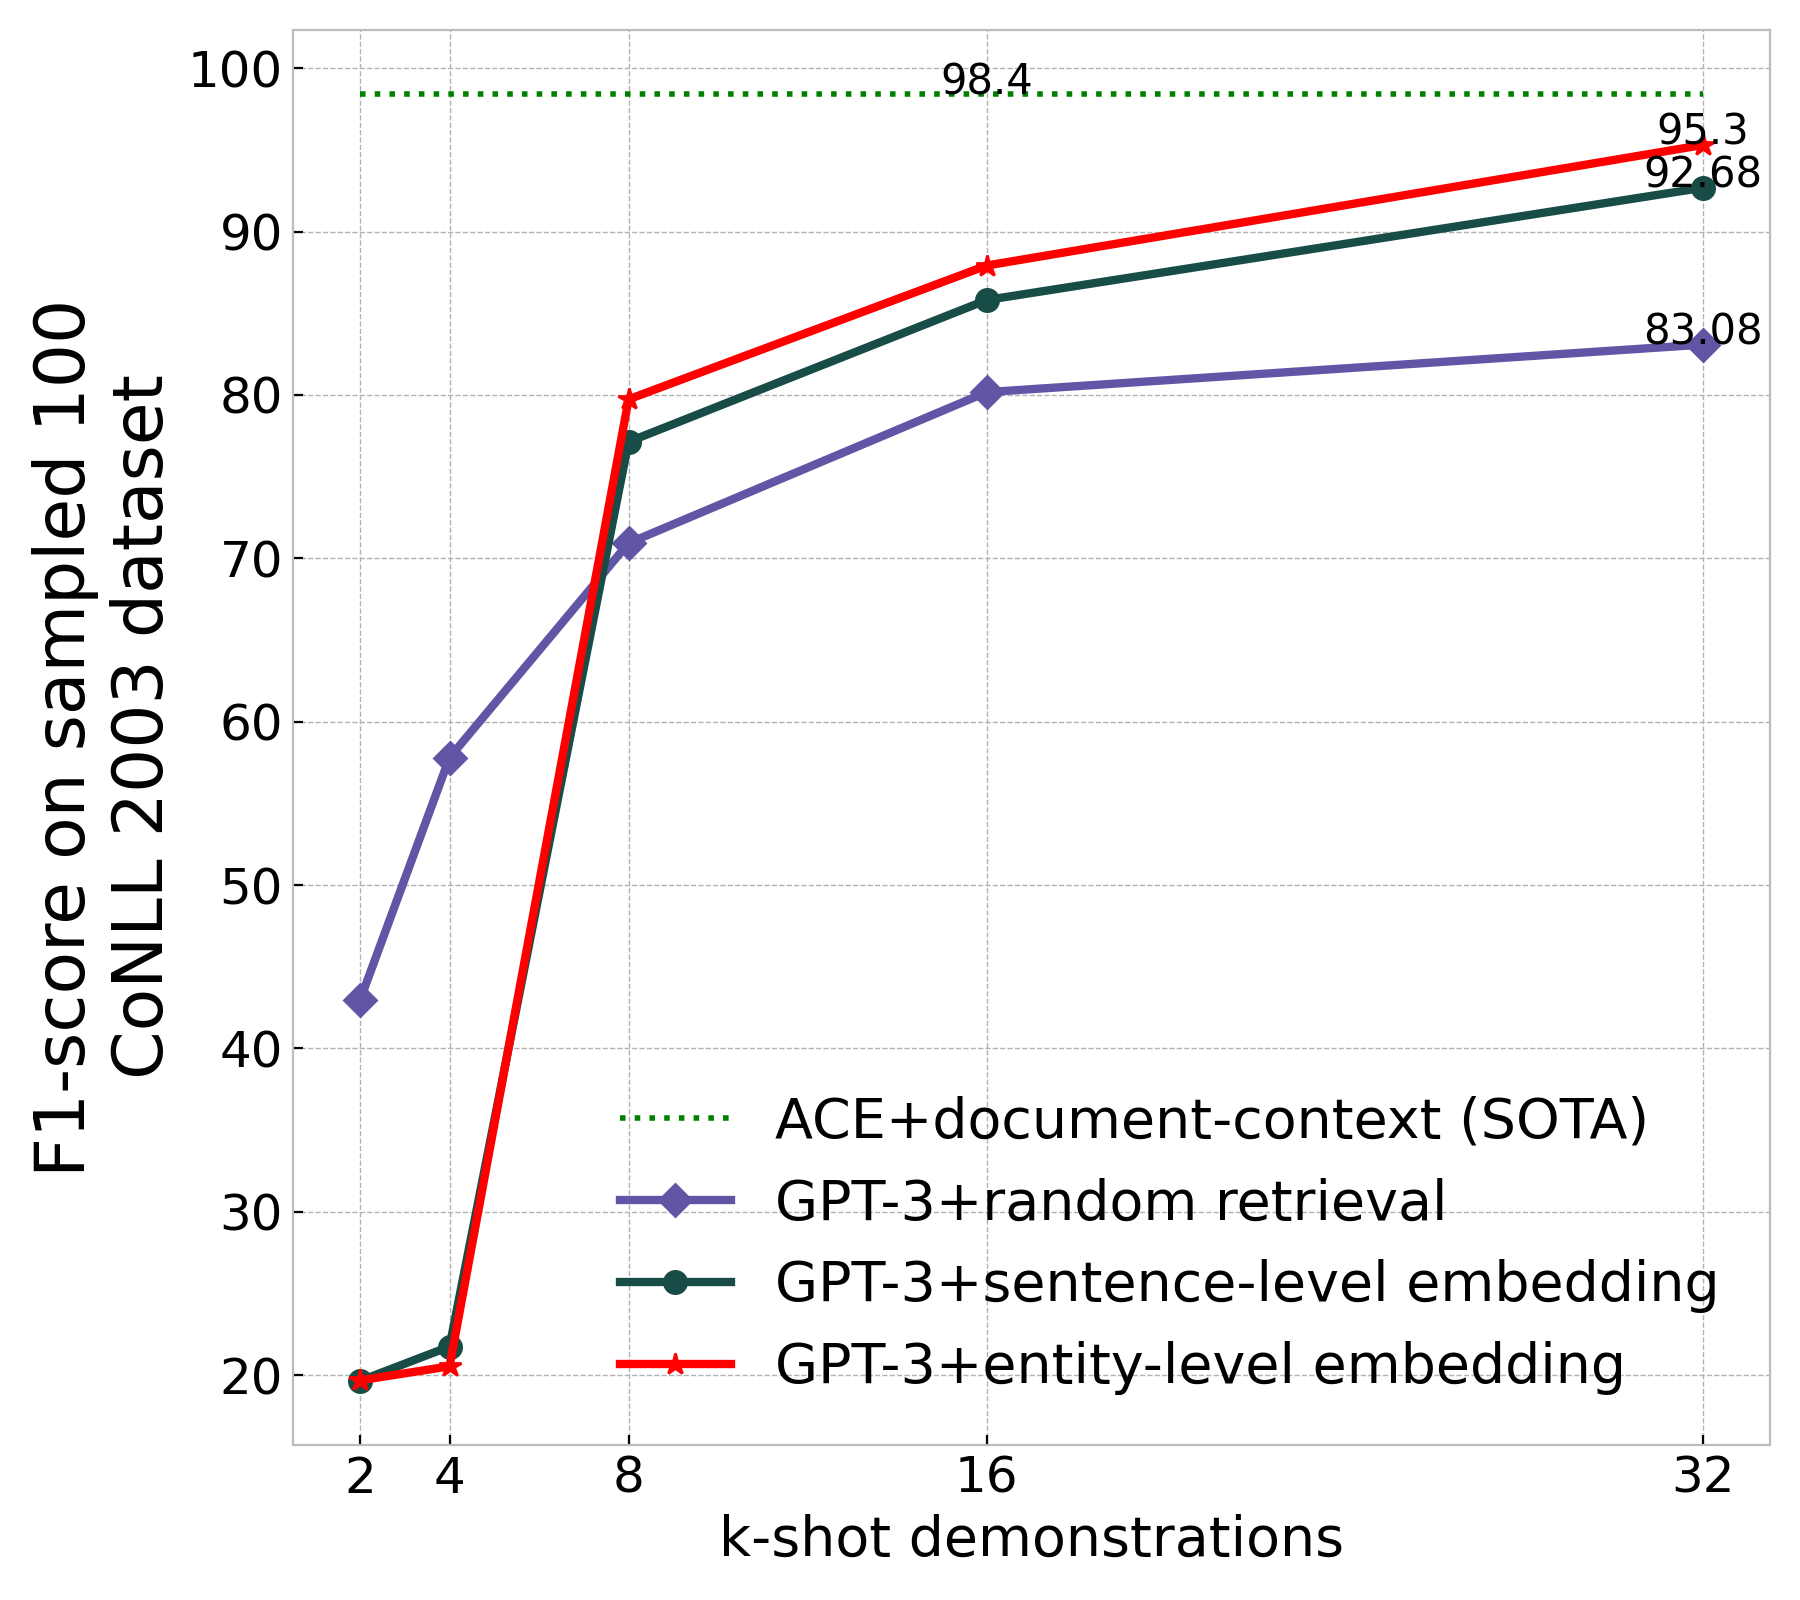
\includegraphics[scale=0.34]{images/k_shot_demonstrations.png}
    \caption{变化$k$-shot演示的对比。}
    \label{fig:k_shot_demonstrations}
\end{figure}

\section{结论}

本文提出GPT-NER来适配LLM到NER任务。为弥合序列标注任务与文本生成任务之间的差距，我们指导LLM通过用特殊标记包围实体来生成标记序列。此外，我们提出自验证策略来缓解LLM模型的幻觉问题。我们在平面和嵌套NER数据集上进行了实验，达到了与完全监督基线相当的性能。除此之外，我们发现GPT-NER在低资源场景下具有卓越的能力，当训练数据极其稀缺时，GPT-NER的结果显著优于监督模型。

\newpage
\appendix

\section*{附录}
\addcontentsline{toc}{section}{附录}

\begin{table*}[th!]
    \centering
    \resizebox{\textwidth}{!}{
    \begin{tabular}{ll}\toprule
        \multicolumn{2}{c}{{\bf English CoNLL2003实体标注}} \\ \midrule
        \textbf{实体类型} & \multicolumn{1}{c}{{\bf 标注说明}} \\ \midrule
        \text{ORG} & \text{组织实体限于命名的公司、政府或其他组织实体} \\ \midrule
        \text{PER} & \text{人物实体是命名的人物或家族} \\ \midrule
        \text{LOC} & \text{地点实体是政治或地理定义的位置名称，如城市、省份、国家、国际区域、水域、山脉等} \\ \midrule
        \text{MISC} & \text{其他实体包括事件、国籍、产品和艺术品} \\ \bottomrule
    \end{tabular}
    }
     \caption{平面NER数据集CoNLL2003的实体标注。}
    \label{tab:conll_annotations}
\end{table*}

\begin{table*}[th!]
    \centering
    \resizebox{.5\textwidth}{!}{
    \begin{tabular}{ll}\toprule
        \multicolumn{2}{c}{{\bf English OntoNotes5.0实体标注}} \\ \midrule
        \textbf{实体类型} & \multicolumn{1}{c}{{\bf 标注说明}} \\ \midrule
        \text{PERSON} & \text{人物，包括虚构人物} \\ \midrule
        \text{NORP} & \text{民族或宗教或政治团体} \\ \midrule
        \text{FAC} & \text{建筑物、机场、公路、桥梁等} \\ \midrule
        \text{ORG} & \text{公司、机构、组织等} \\ \midrule
        \text{GPE} & \text{国家、城市、州} \\ \midrule
        \text{LOC} & \text{非GPE地点、山脉、水域} \\ \midrule
        \text{PRODUCT} & \text{车辆、武器、食品等} \\ \midrule
        \text{EVENT} & \text{命名的飓风、战役、战争、体育赛事等} \\ \midrule
        \text{WORK\_OF\_ART} & \text{书籍、歌曲等标题} \\ \midrule
        \text{LAW} & \text{成为法律的命名文件} \\ \midrule
        \text{LANGUAGE} & \text{任何命名的语言} \\ \midrule
        \text{DATE} & \text{绝对或相对日期或时期} \\ \midrule
        \text{TIME} & \text{小于一天的时间} \\ \midrule
        \text{PERCENT} & \text{百分比（包括"\%"）} \\ \midrule
        \text{MONEY} & \text{货币价值，包括单位} \\ \midrule
        \text{QUANTITY} & \text{度量，如重量或距离} \\ \midrule
        \text{ORDINAL} & \text{"first"、"second"等} \\ \midrule
        \text{CARDINAL} & \text{不属于其他类型的数字} \\ \bottomrule
    \end{tabular}
    }
     \caption{平面NER数据集OntoNotes5.0的实体标注。}
    \label{tab:ontonotes_annotations}
\end{table*}

\begin{table}[th!]
    \centering
    \resizebox{.5\textwidth}{!}{
    \begin{tabular}{lccc}\toprule
        \multicolumn{4}{c}{{\bf English CoNLL2003统计信息}} \\ \midrule
        \textbf{数据集} & \textbf{句子数} & \textbf{词元数} & \textbf{实体数}\\ \midrule
        训练集 & 14,987 & 203,621 & 23,499 \\ \midrule
        开发集 & 3,466 & 51,362 & 5,942 \\ \midrule
        测试集 & 3,684 & 46,435 & 5,648 \\ \bottomrule
        \multicolumn{4}{c}{{\bf English OntoNotes5.0统计信息}} \\ \midrule
        \textbf{数据集} & \textbf{句子数} & \textbf{词元数} & \textbf{实体数} \\ \midrule
        训练集 & 59,924 & 1,088,503 & 81,828 \\ \midrule
        开发集 & 8,528 & 147,724 & 11,066 \\ \midrule
        测试集 & 8,262 & 152,728 & 11,257 \\ \bottomrule
    \end{tabular}
    }
     \caption{平面NER数据集English CoNLL2003和OntoNotes5.0的句子数、词元数和实体数。}
    \label{tab:statistics_on_conll}
\end{table}

\begin{table}[th!]
    \centering
    \resizebox{.5\textwidth}{!}{
    \begin{tabular}{lcccc}\toprule
        \multicolumn{5}{c}{{\bf ACE2004统计信息}} \\ \midrule
        \textbf{数据集} & \textbf{句子数} & \textbf{实体数} & \textbf{嵌套实体数} & \textbf{嵌套百分比} \\ \midrule
        训练集 & 6,200 & 22,204 & 10,149 & 45.71\% \\ \midrule
        开发集 & 745 & 2,514 & 1,092 & 46.69\% \\ \midrule
        测试集 & 812 & 3,035 & 1,417 & 45.61\% \\ \bottomrule
        \multicolumn{5}{c}{{\bf ACE2005统计信息}} \\ \midrule
        \textbf{数据集} & \textbf{句子数} & \textbf{实体数} & \textbf{嵌套实体数} & \textbf{嵌套百分比} \\ \midrule
        训练集 & 7,194 & 24,441 & 9,389 & 38.41\% \\ \midrule
        开发集 & 969 & 3,200 & 1,112 & 34.75\% \\ \midrule
        测试集 & 1,047 & 2,993 & 1,118 & 37.35\% \\ \bottomrule
        \multicolumn{5}{c}{{\bf GENIA统计信息}} \\ \midrule
        \textbf{数据集} & \textbf{句子数} & \textbf{实体数} & \textbf{嵌套实体数} & \textbf{嵌套百分比} \\ \midrule
        训练集 & 16,692 & 50,509 & 9,064 & 17.95\% \\ \midrule
        开发集 & - & - & - & - \\ \midrule
        测试集 & 1,854 & 5,506 & 1,199 & 21.78\% \\ \bottomrule
    \end{tabular}
    }
     \caption{嵌套NER数据集ACE2004、ACE2005和GENIA的句子数、实体数、嵌套实体数和嵌套百分比。}
    \label{tab:statistics_on_nested}
\end{table}

\begin{table*}[th!]
    \centering
    \resizebox{\textwidth}{!}{
    \begin{tabular}{ll}\toprule
        \multicolumn{2}{c}{{\bf English ACE2004和ACE2005实体标注}} \\ \midrule
        \textbf{实体类型} & \multicolumn{1}{c}{{\bf 标注说明}} \\ \midrule
        \text{GPE} & \text{地理政治实体是由政治和/或社会群体定义的地理区域，如国家、民族、地区、城市、州、政府及其人民} \\ \midrule
        \text{ORG} & \text{组织实体限于公司、企业、机构、组织和其他人群} \\ \midrule
        \text{PER} & \text{人物实体限于人类，包括个人或群体} \\ \midrule
        \text{FAC} & \text{设施实体限于建筑物和其他永久性人造结构，如建筑物、机场、公路、桥梁} \\ \midrule
        \text{VEH} & \text{交通工具实体是主要用于移动、携带、拉动或推动运输对象的物理装置，如直升机、火车、船舶和摩托车} \\ \midrule
        \text{LOC} & \text{地点实体限于地理实体，如地理区域和陆地、山脉、水域和地质构造} \\ \midrule
        \text{WEA} & \text{武器实体限于物理装置，如用于物理伤害的仪器，如枪支、武器和火药} \\ \bottomrule
    \end{tabular}
    }
     \caption{数据集ACE2004和ACE2005的实体标注。}
    \label{tab:ace_annotations}
\end{table*}

\subsection{平面NER数据集详情}
\label{flat_ner_datasets_details}

\paragraph{CoNLL2003。}CoNLL2003\cite{sang2003introduction}包含四种类型的命名实体：地点、组织、人物和其他。表\ref{tab:conll_annotations}显示了每种实体类型的标注，表\ref{tab:statistics_on_conll}显示了CoNLL2003中的句子数、词元数和实体数。

\paragraph{OntoNotes5.0。}OntoNotes\cite{pradhan2013towards}包含18种类型的命名实体，表\ref{tab:ontonotes_annotations}列出了每种实体及其标注。OntoNotes5.0的句子数、词元数和实体数显示在表\ref{tab:statistics_on_conll}中。

\subsection{嵌套NER数据集详情}
\label{nested_ner_datasets_details}

\paragraph{ACE2004和ACE2005。}ACE2004\cite{doddington2004automatic}和ACE2005\cite{christopher2006ace}是两个英语嵌套NER数据集，包含七种实体类型：地理政治实体（GPE）、组织实体（ORG）、人物实体（PER）、设施实体（FAC）、交通工具实体（VEH）、地点实体（LOC）和武器实体（WEA）。每种实体类型的标注显示在表\ref{tab:ace_annotations}中，句子数、实体数、嵌套实体数和嵌套百分比显示在表\ref{tab:statistics_on_nested}中。

\paragraph{GENIA。}GENIA是分子生物学领域的英语嵌套NER数据集，包含五种实体类型：细胞系、细胞类型、DNA、RNA和蛋白质。从字面上看，每种实体根据生物学意义命名，句子数、实体数、嵌套实体数和嵌套百分比显示在表\ref{tab:statistics_on_nested}中。

\section{BMES和Entity+Position格式的错误案例}
\label{error_format_example}

我们在采样100条的CoNLL2003数据集上选取了若干示例，以更好地说明BMES和Entity+Position这两种格式的无效性。BMES格式如表\ref{tab:bmes_format}所示，Entity+Position格式如表\ref{tab:entity_position_format}所示。

从这些示例中，我们可以明显观察到：(1) 对于BMES格式，GPT-3难以生成与输入句子长度相同的输出，特别是当输入句子较长时；(2) 对于Entity+Position格式，GPT-3容易混淆位置信息的含义。

\begin{table*}[th!]
    \centering
    \resizebox{\textwidth}{!}{
    \begin{tabular}{l}\toprule
       	\textbf{示例1 {\color{red} 长度错误}} \\\midrule
       	\textit{任务描述} \\
       	我是一位优秀的语言学家。任务是标注组织实体。以下是一些示例。 \\\midrule
       	\textit{句子级演示} \\
输入: Soccer - results of South Korean PRO-SOCCER games . \\
输出: O O O O O O O O O \\
输入: Soccer - results of South Korean PRO-SOCCER games . \\
输出: O O O O O O O O O \\
输入: Soccer - results of South Korean PRO-SOCCER games . \\
输出: O O O O O O O O O \\
输入: Soccer - Italian cup second round results . \\
输出: O O O O O O O O \\\midrule
\textit{输入句子与GPT-3输出} \\
输入: Soccer - Japan get lucky win , China in surprise defeat . \\
输出: O O O O O O O O O O O \\
{\color{blue}\it 期望输出}: O O O O O O O O O O O O \\\bottomrule

\textbf{示例2 {\color{red} 长度错误和实体错误}} \\\midrule
       	\textit{任务描述} \\
我是一位优秀的语言学家。任务是标注其他实体。以下是一些示例。 \\\midrule
\textit{句子级演示} \\
输入: Soccer - results of South Korean PRO-SOCCER games . \\
输出: O O O O B-MISC E-MISC O O O \\
输入: Soccer - results of South Korean PRO-SOCCER games . \\
输出: O O O O B-MISC E-MISC O O O \\
输入: Soccer - results of South Korean PRO-SOCCER games . \\
输出: O O O O B-MISC E-MISC O O O \\
输入: Soccer - Italian cup second round results . \\
输出: O O B-MISC E-MISC O O O O \\\midrule
\textit{输入句子与GPT-3输出} \\
输入: Soccer - Japan get lucky win , China in surprise defeat . \\
输出: O O B-MISC E-MISC O O O O B-MISC E-MISC O O \\
{\color{blue}\it 期望输出}: O O O O O O O O O O O O \\\bottomrule

\textbf{示例3 {\color{red} 长度错误}} \\\midrule
       	\textit{任务描述} \\
我是一位优秀的语言学家。任务是标注人物实体。以下是一些示例。 \\\midrule
\textit{句子级演示} \\
输入: Dubai 1996-08-26 \\
输出: O O \\
输入: Dubai 1996-08-29 \\
输出: O O \\
输入: Dubai 1996-08-29 \\
输出: O O \\
输入: Dubai 1996-08-22 \\
输出: O O \\\midrule
\textit{输入句子与GPT-3输出} \\
输入: AL-AIN , United Arab Emirates 1996-12-06 \\
输出: O O \\
{\color{blue}\it 期望输出}: O O O O O O \\\bottomrule

\textbf{示例4 {\color{red} 长度错误和实体错误}} \\\midrule
\textit{任务描述} \\
我是一位优秀的语言学家。任务是标注地点实体。以下是一些示例。 \\\midrule
\textit{句子级演示} \\
输入: Azerbaijan beat Switzerland 1-0 ( halftime 1-0 ) in their World Cup soccer European group three qualifying match on Saturday . \\
输出: S-LOC O S-LOC O O O O O O O O O O O O O O O O O O \\
输入: Nijmeh of Lebanon beat Nasr of Saudi Arabia 1-0 ( halftime 1-0 ) in their Asian club championship second round first leg tie on Saturday . \\
输出: O O S-LOC O O O B-LOC E-LOC O O O O O O O O O O O O O O O O O O \\
输入: Slovakia beat the Faroe Islands 2-1 ( halftime 1-0 ) in their World Cup soccer European group six qualifying match on Saturday . \\
输出: S-LOC O O B-LOC E-LOC O O O O O O O O O O O O O O O O O O \\
输入: Canada beat Panama 3-1 ( halftime 2-0 ) in their CONCACAF semifinal phase qualifying match for the 1998 World Cup on Friday . \\
输出: S-LOC O S-LOC O O O O O O O O O O O O O O O O O O O O \\\midrule
\textit{输入句子与GPT-3输出} \\
输入: Japan began the defence of their Asian Cup title with a lucky 2-1 win against Syria in a Group C championship match on Friday . \\
输出: S-LOC O O O O O O O O O O O O B-LOC E-LOC O O O O O O O O O O O O O O \\
{\color{blue}\it 期望输出}: S-LOC O O O O O O O O O O O O O O S-LOC O O O O O O O O O \\\bottomrule
    \end{tabular}
    }
     \caption{BMES输出格式在采样100条CoNLL2003数据集上的示例，错误信息以红色标注，期望的正确输出以蓝色标注。}
    \label{tab:bmes_format}
\end{table*}

\begin{table*}[th!]
    \centering
    \resizebox{\textwidth}{!}{
    \begin{tabular}{l}\toprule
       	\textbf{示例1 {\color{red} 位置错误和实体错误}} \\\midrule
       	\textit{任务描述} \\
我是一位优秀的语言学家。任务是标注其他实体。以下是一些示例。 \\\midrule
\textit{句子级演示} \\
输入: Soccer - results of South Korean PRO-SOCCER games . \\
输出: South Korean(4) \\
输入: Soccer - results of South Korean PRO-SOCCER games . \\
输出: South Korean(4) \\
输入: Soccer - results of South Korean PRO-SOCCER games . \\
输出: South Korean(4) \\
输入: Soccer - Italian cup second round results . \\
输出: Italian cup(2) \\\midrule
\textit{输入句子与GPT-3输出} \\
输入: Soccer - Japan get lucky win , China in surprise defeat . \\
输出: Japan(4), China(4) \\
{\color{blue}\it 期望输出}: None \\\bottomrule

\textbf{示例2 {\color{red} 位置错误和实体错误}} \\\midrule
       	\textit{任务描述} \\
我是一位优秀的语言学家。任务是标注组织实体。以下是一些示例。 \\\midrule
\textit{句子级演示} \\
输入: Dubai 1996-08-26 \\
输出: None \\
输入: Dubai 1996-08-29 \\
输出: None \\
输入: Dubai 1996-08-29 \\
输出: None \\
输入: Dubai 1996-08-22 \\
输出: None \\\midrule
\textit{输入句子与GPT-3输出} \\
输入: AL-AIN , United Arab Emirates 1996-12-06 \\
输出: AL-AIN, United Arab Emirates \\
{\color{blue}\it 期望输出}: None \\\bottomrule

\textbf{示例3 {\color{red} 位置错误}} \\\midrule
       	\textit{任务描述} \\
我是一位优秀的语言学家。任务是标注地点实体。以下是一些示例。 \\\midrule
\textit{句子级演示} \\
输入: Third seed Arantxa Sanchez Vicario , the 1994 champion , and eighth-seeded Olympic gold medalist Lindsay Davenport dropped three game each en route to the second round . \\
输出: None \\
输入: Dutch champions Ajax Amsterdam faltered in their second league match of the season on Saturday losing 2-0 away at Heerenveen . \\
输出: None \\
输入: Soccer - disappointing Ajax slump 2-0 at Heerenveen . \\
输出: Heerenveen(7) \\
输入: Australian Open runner-up Anke Huber of Germany , the sixth seed , was undone by an unlucky draw that put her against 17th ranked South African Amanda Coetzer in her opening match . \\
输出: Germany(6) \\\midrule
\textit{输入句子与GPT-3输出} \\
输入: But China saw their luck desert them in the second match of the group , crashing to a surprise 2-0 defeat to newcomers Uzbekistan . \\
输出: China(2), Uzbekistan(9) \\
{\color{blue}\it 期望输出}: China(1), Uzbekistan(23) \\\bottomrule

\textbf{示例4 {\color{red} 位置错误和实体错误}} \\\midrule
\textit{任务描述} \\
我是一位优秀的语言学家。任务是标注其他实体。以下是一些示例。 \\
\textit{句子级演示} \\
输入: Azerbaijan beat Switzerland 1-0 ( halftime 1-0 ) in their World Cup soccer European group three qualifying match on Saturday . \\
输出: World Cup(10), European(13) \\
输入: Nijmeh of Lebanon beat Nasr of Saudi Arabia 1-0 ( halftime 1-0 ) in their Asian club championship second round first leg tie on Saturday . \\
输出: Asian(15) \\
输入: Slovakia beat the Faroe Islands 2-1 ( halftime 1-0 ) in their World Cup soccer European group six qualifying match on Saturday . \\
输出: World Cup(12), European(15) \\
输入: Canada beat Panama 3-1 ( halftime 2-0 ) in their CONCACAF semifinal phase qualifying match for the 1998 World Cup on Friday . \\
输出: World Cup(18) \\\midrule
\textit{输入句子与GPT-3输出} \\
输入: Japan began the defence of their Asian Cup title with a lucky 2-1 win against Syria in a Group C championship match on Friday . \\
输出: Asian(14) \\
{\color{blue}\it 期望输出}: Asian Cup(6) \\\bottomrule
    \end{tabular}
    }
     \caption{Entity+Position输出格式在采样100条CoNLL2003数据集上的示例，错误信息以红色标注，期望的正确输出以蓝色标注。}
    \label{tab:entity_position_format}
\end{table*}

\section{演示示例}
\label{demonstrations_examples}

为了更好地说明GPT-NER的演示效果，我们在表\ref{tab:example_random_retrieval_embedding}中选取了随机检索的若干示例，在表\ref{tab:example_sentence_level_embedding}中选取了句子级嵌入的示例，在表\ref{tab:example_entity_level_embedding}中选取了实体级嵌入的示例。从这些结果中，我们可以观察到：

(1) 对于表\ref{tab:example_random_retrieval_embedding}中的随机检索，我们可以观察到所有句子都有同等机会作为少样本演示中的示例出现，且输入句子与每个检索到的示例通常不包含相似的示例。

(2) 对于表\ref{tab:example_sentence_level_embedding}中的句子级嵌入，我们可以观察到检索到的示例与输入句子的语义相似，但可能不关注与输入句子相同的局部实体。

(3) 对于表\ref{tab:example_entity_level_embedding}中的实体级嵌入，我们可以观察到检索到的示例确实关注与输入句子相同的局部实体，从而使GPT-3的预测过程更加容易。这一现象强调了少样本学习中演示质量的有效性。

\begin{table*}[th!]
    \centering
    \resizebox{\textwidth}{!}{
    \begin{tabular}{l}\toprule
       	\textbf{示例1} \\\midrule
       	\textit{任务描述} \\
我是一位优秀的语言学家。任务是标注其他实体。以下是一些示例。 \\\midrule
\textit{句子级演示} \\
输入: Seattle at Boston \\
输出: Seattle at Boston \\
输入: 3. Carla Sacramento ( Portugal ) 4:08.96 \\
输出: 3. Carla Sacramento ( Portugal ) 4:08.96 \\
输入: Director Budge Weidman , who has shepherded the project from the beginning , predicts it will take up to a decade to complete . \\
输出: Director Budge Weidman , who has shepherded the project from the beginning , predicts it will take up to a decade to complete . \\
输入: Hull 0 Barnet 0 \\
输出: Hull 0 Barnet 0 \\
输入: Scott Draper ( Australia ) vs. Galo Blanco ( Spain ) \\
输出: Scott Draper ( Australia ) vs. Galo Blanco ( Spain ) \\
输入: Standings in the French first \\
输出: Standings in the @@French\#\# first \\
输入: He said only the removal of the government and an early election could save Pakistan from disaster . " \\
输出: He said only the removal of the government and an early election could save Pakistan from disaster . " \\
输入: Stock markets \\
输出: Stock markets \\\midrule
\textit{输入句子与GPT-3输出} \\
输入: Soccer - Japan get lucky win , China in surprise defeat . \\
输出: Soccer - Japan get lucky win , China in surprise defeat . \\
{\color{blue}\it 期望输出}: Soccer - Japan get lucky win , China in surprise defeat . \\\bottomrule

\textbf{示例2} \\\midrule
       	\textit{任务描述} \\
我是一位优秀的语言学家。任务是标注组织实体。以下是一些示例。 \\\midrule
\textit{句子级演示} \\
输入: Jakob Hlasek ( Switzerland ) beat Alberto Berasategui ( Spain ) 7-6 ( 7-5 ) 7-6 ( 9-7 ) 6-0 \\
输出: Jakob Hlasek ( Switzerland ) beat Alberto Berasategui ( Spain ) 7-6 ( 7-5 ) 7-6 ( 9-7 ) 6-0 \\
输入: After bogeying the 10th hole to move to four-over for the round , he rallied for birdies on 15 and 18 . \\
输出: After bogeying the 10th hole to move to four-over for the round , he rallied for birdies on 15 and 18 . \\
输入: Abidjan 1996-08-29 \\
输出: Abidjan 1996-08-29 \\
输入: Falkirk 1 Partick 0 \\
输出: @@Falkirk\#\# 1 @@Partick\#\# 0 \\
输入: Williams seized two wickets in two deliveries and left-armer Ilott also captured two as Gloucestershire , 252 behind on first innings , slumped to 27 for four at the close on the third day of the four-day game at Colchester . \\
输出: Williams seized two wickets in two deliveries and left-armer Ilott also captured two as @@Gloucestershire\#\# , 252 behind on first innings , slumped to 27 for four at the close on the third day of the four-day game at Colchester . \\
输入: South Queensland 21 4 0 17 210 460 8 \\
输出: @@South Queensland\#\# 21 4 0 17 210 460 8 \\
输入: In Skopje : Sloga Jugomagnat ( Macedonia ) 0 Kispest Honved \\
输出: In Skopje : @@Sloga Jugomagnat\#\# ( Macedonia ) 0 Kispest Honved \\
输入: Call C 98.00 pct 0.47 Dem 3.30 pct 202.90 X \\
输出: Call C 98.00 pct 0.47 Dem 3.30 pct 202.90 X \\\midrule
\textit{输入句子与GPT-3输出} \\
输入: AL-AIN , United Arab Emirates 1996-12-06 \\
输出: @@AL-AIN\#\# , United Arab Emirates 1996-12-06 \\
{\color{blue}\it 期望输出}: AL-AIN , United Arab Emirates 1996-12-06 \\\bottomrule

\textbf{示例3} \\\midrule
       	\textit{任务描述} \\
我是一位优秀的语言学家。任务是标注其他实体。以下是一些示例。 \\\midrule
\textit{句子级演示} \\
输入: Serbian policeman shot dead in Kosovo province . \\
输出: @@Serbian\#\# policeman shot dead in Kosovo province . \\
输入: British Labour Party leader Tony Blair won a narrow victory on Saturday when the party 's Scottish executive voted 21-18 in favour of his plans for a referendum on a separate parliament for Scotland . \\
输出: British Labour Party leader Tony Blair won a narrow victory on Saturday when the party 's @@Scottish\#\# executive voted 21-18 in favour of his plans for a referendum on a separate parliament for Scotland . \\
输入: Newcastle 24 Western Reds 20 \\
输出: Newcastle 24 Western Reds 20 \\
输入: WSRL is part of the Welspun group which has a presence in the cotton yarn , terry towels and polyester yarn industry , the statement said . \\
输出: WSRL is part of the Welspun group which has a presence in the cotton yarn , terry towels and polyester yarn industry , the statement said . \\
输入: In Chicago , Erik Hanson outdueled Alex Fernandez , and Jacob Brumfield drove in Otis Nixon with the game 's only run in the sixth inning as the Toronto Blue Jays blanked the White Sox 1-0 in a game shortened to six innings due to rain . \\
输出: In Chicago , Erik Hanson outdueled Alex Fernandez , and Jacob Brumfield drove in Otis Nixon with the game 's only run in the sixth inning as the Toronto Blue Jays blanked the White Sox 1-0 in a game shortened to six innings due to rain . \\
输入: ( Corrects that Habsudova is sixth seed ) . \\
输出: ( Corrects that Habsudova is sixth seed ) . \\
输入: San Francisco at New York \\
输出: San Francisco at New York \\
输入: -- The short-term price objective is \$ 5 a share and the long-term objective is \$ 9 . \\
输出: -- The short-term price objective is \$ 5 a share and the long-term objective is \$ 9 . \\\midrule
\textit{输入句子与GPT-3输出} \\
输入: Japan began the defence of their Asian Cup title with a lucky 2-1 win against Syria in a Group C championship match on Friday . \\
输出: Japan began the defence of their @@Asian\#\# Cup title with a lucky 2-1 win against @@Syria\#\# in a Group C championship match on Friday . \\
{\color{blue}\it 期望输出}: Japan began the defence of their @@Asian Cup\#\# title with a lucky 2-1 win against Syria in a Group C championship match on Friday . \\\bottomrule
    \end{tabular}
    }
     \caption{使用随机检索在CoNLL2003数据集上的示例。}
    \label{tab:example_random_retrieval_embedding}
\end{table*}

\begin{table*}[th!]
    \centering
    \resizebox{\textwidth}{!}{
    \begin{tabular}{l}\toprule
       	\textbf{示例1} \\\midrule
       	\textit{任务描述} \\
我是一位优秀的语言学家。任务是标注地点实体。以下是一些示例。 \\\midrule
\textit{句子级演示} \\
输入: Dubai 1996-08-26 \\
输出: @@Dubai\#\# 1996-08-26 \\
输入: Dubai 1996-08-29 \\
输出: @@Dubai\#\# 1996-08-29 \\
输入: Dubai 1996-08-29 \\
输出: @@Dubai\#\# 1996-08-29 \\
输入: Dubai 1996-08-22 \\
输出: @@Dubai\#\# 1996-08-22 \\
输入: Dubai 1996-08-25 \\
输出: @@Dubai\#\# 1996-08-25 \\
输入: Baghdad 1996-08-24 \\
输出: @@Baghdad\#\# 1996-08-24 \\
输入: Baghdad 1996-08-27 \\
输出: @@Baghdad\#\# 1996-08-27 \\
输入: Baghdad 1996-08-28 \\
输出: @@Baghdad\#\# 1996-08-28 \\\midrule
\textit{输入句子与GPT-3输出} \\
输入: AL-AIN , United Arab Emirates 1996-12-06 \\
输出: @@AL-AIN\#\# , @@United Arab Emirates\#\# 1996-12-06 \\
{\color{blue}\it 期望输出}: @@AL-AIN\#\# , @@United Arab Emirates\#\# 1996-12-06 \\\bottomrule

\textbf{示例2} \\\midrule
       	\textit{任务描述} \\
我是一位优秀的语言学家。任务是标注地点实体。以下是一些示例。 \\\midrule
\textit{句子级演示} \\
输入: Azerbaijan beat Switzerland 1-0 ( halftime 1-0 ) in their World Cup soccer European group three qualifying match on Saturday . \\
输出: @@Azerbaijan\#\# beat @@Switzerland\#\# 1-0 ( halftime 1-0 ) in their World Cup soccer European group three qualifying match on Saturday . \\
输入: Nijmeh of Lebanon beat Nasr of Saudi Arabia 1-0 ( halftime 1-0 ) in their Asian club championship second round first leg tie on Saturday . \\
输出: Nijmeh of @@Lebanon\#\# beat Nasr of @@Saudi Arabia\#\# 1-0 ( halftime 1-0 ) in their Asian club championship second round first leg tie on Saturday . \\
输入: Slovakia beat the Faroe Islands 2-1 ( halftime 1-0 ) in their World Cup soccer European group six qualifying match on Saturday . \\
输出: @@Slovakia\#\# beat the @@Faroe Islands\#\# 2-1 ( halftime 1-0 ) in their World Cup soccer European group six qualifying match on Saturday . \\
输入: Canada beat Panama 3-1 ( halftime 2-0 ) in their CONCACAF semifinal phase qualifying match for the 1998 World Cup on Friday . \\
输出: @@Canada\#\# beat @@Panama\#\# 3-1 ( halftime 2-0 ) in their CONCACAF semifinal phase qualifying match for the 1998 World Cup on Friday . \\
输入: Soccer - Azerbaijan beat Switzerland in world cup Qualifier . \\
输出: Soccer - @@Azerbaijan\#\# beat @@Switzerland\#\# in world cup Qualifier . \\
输入: Soccer - Wales beat San Marino in world cup Qualifier . \\
输出: Soccer - @@Wales\#\# beat @@San Marino\#\# in world cup Qualifier . \\
输入: The United States edged Austria in Salzburg 3-2 in the opening round in April , and then blanked Japan 5-0 in Nagoya last month in the semifinals . \\
输出: The @@United States\#\# edged @@Austria\#\# in @@Salzburg\#\# 3-2 in the opening round in April , and then blanked @@Japan\#\# 5-0 in @@Nagoya\#\# last month in the semifinals . \\
输入: Soccer - Slovakia beat Faroes in world cup Qualifier . \\
输出: Soccer - @@Slovakia\#\# beat @@Faroes\#\# in world cup Qualifier . \\\midrule
\textit{输入句子与GPT-3输出} \\
输入: Japan began the defence of their Asian Cup title with a lucky 2-1 win against Syria in a Group C championship match on Friday . \\
输出: @@Japan\#\# began the defence of their Asian Cup title with a lucky 2-1 win against @@Syria\#\# in a Group C championship match on Friday .\\
{\color{blue}\it 期望输出}: @@Japan\#\# began the defence of their Asian Cup title with a lucky 2-1 win against @@Syria\#\# in a Group C championship match on Friday . \\\bottomrule

\textbf{示例3} \\\midrule
       	\textit{任务描述} \\
我是一位优秀的语言学家。任务是标注其他实体。以下是一些示例。 \\\midrule
\textit{句子级演示} \\
输入: Azerbaijan beat Switzerland 1-0 ( halftime 1-0 ) in their World Cup soccer European group three qualifying match on Saturday . \\
输出: Azerbaijan beat Switzerland 1-0 ( halftime 1-0 ) in their @@World Cup\#\# soccer @@European\#\# group three qualifying match on Saturday . \\
输入: Nijmeh of Lebanon beat Nasr of Saudi Arabia 1-0 ( halftime 1-0 ) in their Asian club championship second round first leg tie on Saturday . \\
输出: Nijmeh of Lebanon beat Nasr of Saudi Arabia 1-0 ( halftime 1-0 ) in their @@Asian\#\# club championship second round first leg tie on Saturday . \\
输入: Slovakia beat the Faroe Islands 2-1 ( halftime 1-0 ) in their World Cup soccer European group six qualifying match on Saturday . \\
输出: Slovakia beat the Faroe Islands 2-1 ( halftime 1-0 ) in their @@World Cup\#\# soccer @@European\#\# group six qualifying match on Saturday . \\
输入: Canada beat Panama 3-1 ( halftime 2-0 ) in their CONCACAF semifinal phase qualifying match for the 1998 World Cup on Friday . \\
输出: Canada beat Panama 3-1 ( halftime 2-0 ) in their CONCACAF semifinal phase qualifying match for the 1998 @@World Cup\#\# on Friday . \\
输入: Soccer - Azerbaijan beat Switzerland in world cup Qualifier . \\
输出: Soccer - Azerbaijan beat Switzerland in @@world cup\#\# Qualifier . \\
输入: Soccer - Wales beat San Marino in world cup Qualifier . \\
输出: Soccer - Wales beat San Marino in @@world cup\#\# Qualifier . \\
输入: The United States edged Austria in Salzburg 3-2 in the opening round in April , and then blanked Japan 5-0 in Nagoya last month in the semifinals . \\
输出: The United States edged Austria in Salzburg 3-2 in the opening round in April , and then blanked Japan 5-0 in Nagoya last month in the semifinals . \\
输入: Soccer - Slovakia beat Faroes in world cup Qualifier . \\
输出: Soccer - Slovakia beat Faroes in @@world cup\#\# Qualifier . \\\midrule
\textit{输入句子与GPT-3输出} \\
输入: Japan began the defence of their Asian Cup title with a lucky 2-1 win against Syria in a Group C championship match on Friday . \\
输出: Japan began the defence of their @@Asian Cup\#\# title with a lucky 2-1 win against Syria in a Group C championship match on Friday . \\
{\color{blue}\it 期望输出}: Japan began the defence of their @@Asian Cup\#\# title with a lucky 2-1 win against Syria in a Group C championship match on Friday . \\\bottomrule

    \end{tabular}
    }
     \caption{使用句子级嵌入在CoNLL2003数据集上的示例。}
    \label{tab:example_sentence_level_embedding}
\end{table*}

\begin{table*}[th!]
    \centering
    \resizebox{\textwidth}{!}{
    \begin{tabular}{l}\toprule
       	\textbf{示例1} \\\midrule
       	\textit{任务描述} \\
我是一位优秀的语言学家。任务是标注地点实体。以下是一些示例。 \\\midrule
\textit{句子级演示} \\
输入: AL-RAM , West Bank 1996-08-30 \\
输出: @@AL-RAM\#\# , @@West Bank\#\# 1996-08-30 \\
输入: AL-MUNTAR , West Bank 1996-08-26 \\
输出: @@AL-MUNTAR\#\# , @@West Bank\#\# 1996-08-26 \\
输入: Teravainen ( U.S. ) , Jean Van de Velde ( France ) , Oyvind Rojahn \\
输出: Teravainen ( @@U.S.\#\# ) , Jean Van de Velde ( @@France\#\# ) , Oyvind Rojahn \\
输入: The greatest declines in the volume of help-wanted advertising were in the New England , Mountain and West South Central regions . \\
输出: The greatest declines in the volume of help-wanted advertising were in the @@New England\#\# , @@Mountain\#\# and @@West South Central\#\# regions . \\
输入: Doug Flach ( U.S. ) beat Gianluca Pozzi ( Italy ) 7-5 7-6 ( 7-5 ) 2-6 7-6 ( 8-6 ) \\
输出: Doug Flach ( @@U.S.\#\# ) beat Gianluca Pozzi ( @@Italy\#\# ) 7-5 7-6 ( 7-5 ) 2-6 7-6 ( 8-6 ) \\
输入: Jeff Tarango ( U.S. ) beat Alex Radulescu ( Romania ) 6-7 ( 5-7 ) 6-4 6-1 retired , heat exhaustion \\
输出: Jeff Tarango ( @@U.S.\#\# ) beat Alex Radulescu ( @@Romania\#\# ) 6-7 ( 5-7 ) 6-4 6-1 retired , heat exhaustion \\
输入: Chelsea , 16 , was at President Bill Clinton 's side as he rode the rails through parts of West Virginia , Kentucky and Ohio , and was introduced at every stop . \\
输出: Chelsea , 16 , was at President Bill Clinton 's side as he rode the rails through parts of @@West Virginia\#\# , @@Kentucky\#\# and @@Ohio\#\# , and was introduced at every stop . \\
输入: Clinton said on Saturday he had ordered U.S. forces in the Gulf to go on high alert and was reinforcing them in response to Iraqi attacks on Kurdish dissidents in northern Iraq . \\
输出: Clinton said on Saturday he had ordered @@U.S.\#\# forces in the @@Gulf\#\# to go on high alert and was reinforcing them in response to Iraqi attacks on Kurdish dissidents in northern @@Iraq\#\# . \\\midrule
\textit{输入句子与GPT-3输出} \\
输入: AL-AIN , United Arab Emirates 1996-12-06 \\
输出: @@AL-AIN\#\# , @@United Arab Emirates\#\# 1996-12-06 \\
{\color{blue}\it 期望输出}: @@AL-AIN\#\# , @@United Arab Emirates\#\# 1996-12-06 \\\bottomrule

\textbf{示例2} \\\midrule
       	\textit{任务描述} \\
我是一位优秀的语言学家。任务是标注其他实体。以下是一些示例。 \\\midrule
\textit{句子级演示} \\
输入: The armed hijackers of the Airbus 310 Flight 150 , which is expected to arrive about 4 a.m. ( 0300 GMT ) , have said they intend to surrender and seek political asylum in Britain . \\
输出: The armed hijackers of the @@Airbus 310\#\# @@Flight 150\#\# , which is expected to arrive about 4 a.m. ( 0300 @@GMT\#\# ) , have said they intend to surrender and seek political asylum in Britain . \\
输入: Toronto-based Barrick , the world 's third largest gold producer , sweetened its July 11 bid to C\$ 30 a share from C\$ 27 on August 16 after a fresh batch of drill results from the Pierina deposit . \\
输出: @@Toronto-based\#\# Barrick , the world 's third largest gold producer , sweetened its July 11 bid to @@C\$\#\# 30 a share from @@C\$\#\# 27 on August 16 after a fresh batch of drill results from the Pierina deposit . \\
输入: The club , who put Manchester United out of last year 's UEFA Cup , were fined \$ 1,000 . \\
输出: The club , who put Manchester United out of last year 's @@UEFA Cup\#\# , were fined \$ 1,000 . \\
输入: Shr C\$ 0.12 C\$ 0.15 \\
输出: Shr @@C\$\#\# 0.12 @@C\$\#\# 0.15 \\
输入: Shr C\$ 0.04 C\$ 0.08 \\
输出: Shr @@C\$\#\# 0.04 @@C\$\#\# 0.08 \\
输入: An Iraqi Kurdish group on Wednesday said it had agreed a new U.S.-brokered ceasefire with a rival faction after a previous accord was shattered by sporadic fighting between the groups in recent days . \\
输出: An @@Iraqi Kurdish\#\# group on Wednesday said it had agreed a new @@U.S.-brokered\#\# ceasefire with a rival faction after a previous accord was shattered by sporadic fighting between the groups in recent days . \\
输入: On Friday , Metro Holdings topped gainers , soaring by S\$ 1.55 to close at S\$ 6.05 on market rumours of a takeover bid by First Capital Corp . \\
输出: On Friday , Metro Holdings topped gainers , soaring by @@S\$\#\# 1.55 to close at @@S\$\#\# 6.05 on market rumours of a takeover bid by First Capital Corp . \\
输入: We 're looking for it to stabilise now , " said one Euromark options trader at a U.S. bank . \\
输出: We 're looking for it to stabilise now , " said one @@Euromark\#\# options trader at a U.S. bank . \\\midrule
\textit{输入句子与GPT-3输出} \\
输入: Japan began the defence of their Asian Cup title with a lucky 2-1 win against Syria in a Group C championship match on Friday . \\
输出: Japan began the defence of their @@Asian Cup\#\# title with a lucky 2-1 win against Syria in a Group C championship match on Friday .\\
{\color{blue}\it 期望输出}: Japan began the defence of their @@Asian Cup\#\# title with a lucky 2-1 win against Syria in a Group C championship match on Friday . \\\bottomrule

\textbf{示例3} \\\midrule
       	\textit{任务描述} \\
我是一位优秀的语言学家。任务是标注地点实体。以下是一些示例。 \\\midrule
\textit{句子级演示} \\
输入: In April , China quashed a draft resolution by the U.N. Human Rights Commission expressing concern over continuing reports of Beijing 's violations of fundamental freedoms . \\
输出: In April , @@China\#\# quashed a draft resolution by the U.N. Human Rights Commission expressing concern over continuing reports of @@Beijing\#\# 's violations of fundamental freedoms . \\
输入: China thanks Gabon for support on human rights . \\
输出: @@China\#\# thanks @@Gabon\#\# for support on human rights . \\
输入: China says Taiwan spoils atmosphere for talks . \\
输出: @@China\#\# says @@Taiwan\#\# spoils atmosphere for talks . \\
输入: Asked what India would do if the pact were forwarded to the United Nations General Assembly , Gujral said : " That bridge I will cross when I come to it . " \\
输出: Asked what @@India\#\# would do if the pact were forwarded to the United Nations General Assembly , Gujral said : " That bridge I will cross when I come to it . " \\
输入: China says militant Japan must face war past . \\
输出: @@China\#\# says militant @@Japan\#\# must face war past . \\
输入: The victory against Japan marked the Fed Cup debut of Monica Seles , who became a naturalised U.S. citizen in 1994 . \\
输出: The victory against @@Japan\#\# marked the Fed Cup debut of Monica Seles , who became a naturalised @@U.S.\#\# citizen in 1994 . \\
输入: The constitutional monarch , who last visited China in 1993 , was scheduled to meet Chinese President Jiang Zemin and Premier Li Peng during his visit , they said . \\
输出: The constitutional monarch , who last visited @@China\#\# in 1993 , was scheduled to meet Chinese President Jiang Zemin and Premier Li Peng during his visit , they said . \\
输入: Atheist China officially bans missionary activities but often turns a blind eye to religious activities of people nominally employed as foreign language teachers , particularly in remote areas that are unable to attract other candidates . \\
输出: Atheist @@China\#\# officially bans missionary activities but often turns a blind eye to religious activities of people nominally employed as foreign language teachers , particularly in remote areas that are unable to attract other candidates . \\\midrule
\textit{输入句子与GPT-3输出} \\
输入: But China saw their luck desert them in the second match of the group , crashing to a surprise 2-0 defeat to newcomers Uzbekistan . \\
输出: But @@China\#\# saw their luck desert them in the second match of the group , crashing to a surprise 2-0 defeat to newcomers @@Uzbekistan\#\# \\
{\color{blue}\it 期望输出}: But @@China\#\# saw their luck desert them in the second match of the group , crashing to a surprise 2-0 defeat to newcomers @@Uzbekistan\#\#  \\\bottomrule
    \end{tabular}
    }
     \caption{使用实体级嵌入在CoNLL2003数据集上的示例。}
    \label{tab:example_entity_level_embedding}
\end{table*}

\bibliography{GPT-NER}

\end{document}
